
\chapter{群的线性表示理论}
\section{群的线性表示}
到目前为止，我们所讨论的群都是抽象的代数结构。为了应用群论来解决物理等领域的具体问题，我们需要一种方法将这些抽象的群元及其运算规则“翻译”成我们熟悉的数学语言。线性表示理论就是实现这一目标的最重要工具。

那么，\textbf{什么是群的表示 (Representation)}？
从本质上讲，一个群 G 的表示，就是找到了另一个我们更熟悉的群 G'（通常是一个矩阵群），并建立了一个从 G 到 G' 的\textbf{同态映射}。
$$
    G \sim G'
$$
通过这个同态映射，原群 G 中复杂的、抽象的乘法关系，就被翻译成了 G' 中具体的、可计算的矩阵乘法关系。


\begin{itemize}
    \item 如果这个同态映射是一个\textbf{同构映射} ($G \cong G'$)，那么这个表示是“忠实”的，称为\textbf{忠实表示 (Faithful Representation)}。
    \item 如果同构映射中的 G' 是一个矩阵群，那么这个表示就是一个\textbf{忠实的矩阵表示}。
\end{itemize}

\subsection{群的线性表示的定义}
\begin{definition}{群的 m 维线性表示}
    假设 $G=\{g_i\}$ 是一个抽象群。如果存在一个映射 D，它为 G 中的每一个元素 $g_i$ 都指定了一个 $m \times m$ 的\textcolor{red}{非奇异矩阵} $D(g_i)$，并且这个映射保持群的乘法结构，即构成一个\textbf{群同态}：
    $$
        \forall g_i, g_j \in G, \quad D(g_i g_j) = D(g_i)D(g_j)
    $$
    则称这组矩阵 $\{D(g_i) \mid g_i \in G\}$ 构成了群 G 的一个 \textbf{m 维线性表示}。
    
    这组表示矩阵自身也构成一个群，我们称之为\textbf{表示群}。
    
    所以，一个 m 维线性表示本质上就是一个从抽象群 G 到 m 维一般线性群 $GL(m)$ 的一个子群的同态映射。
    $$
        g_i \longrightarrow D(g_i)
    $$
    $$
        G \sim \{D(g_i)\} \subseteq GL(m)
    $$
\end{definition}
\begin{remark}
    如果这个表示同态的核 $I = \{g \in G \mid D(g) = E\}$ (E是单位矩阵) 不是平庸的 $\{e\}$，那么这个表示就不是忠实的。根据第一同构定理，此时表示群与商群 $G/I$ 同构：
    $$
        \{D(g_i)\} \cong G/I
    $$
\end{remark}


\subsection{表示的存在性与平庸表示}
一个基本的问题是：是否对于每一个抽象群 G，我们都能为它找到至少一个线性表示？答案是肯定的。存在一种构造方式，它适用于任何群，无论其结构多么复杂。这种表示称为\textbf{平庸表示}。

\begin{definition}{平庸表示 (Trivial Representation)}
    对于任意一个群 $G=\{g_i\}$，其\textbf{平庸表示} D 是一个一维表示，它将 G 中的\textcolor{red}{所有元素}都映射到数字 1 (即 $1 \times 1$ 的单位矩阵)。
    $$
        \forall g_i \in G, \quad D(g_i) = [1]
    $$
\end{definition}

\begin{proof}[验证这是一个合法的表示]
    我们只需验证这个映射是否满足同态条件 $D(g_i g_j) = D(g_i)D(g_j)$。
    \begin{itemize}
        \item 等式左边：由于 $g_i g_j$ 仍然是 G 中的一个元素，所以 $D(g_i g_j) = [1]$。
        \item 等式右边：$D(g_i)D(g_j) = [1] \cdot [1] = [1]$。
    \end{itemize}
    等式两边相等，同态条件满足。因此，平庸表示是一个合法的群表示。
\end{proof}

\begin{note}{平庸表示的性质}
    \begin{itemize}
        \item \textbf{普遍性}: 任何群都拥有平庸表示，它是最基本的存在性证明。
        \item \textbf{非忠实性}: 除非 G 本身是只包含一个元素的平庸群 $\{e\}$，否则平庸表示都是非忠实的。因为它把所有不同的群元都映射到了同一个矩阵 [1]，丢失了群内部的所有结构信息。
        \item \textbf{同态核}: 平庸表示的同态核是整个群 G，即 $I = G$。
        \item \textbf{推广}: 我们可以将平庸表示推广到任意维度 $n$。即把所有群元都映射到 $n \times n$ 的单位矩阵 $E_n$。这也是一个合法的、但非忠实的表示。
    \end{itemize}
\end{note}





\subsection{忠实表示与非忠实表示}
我们已经知道，群的表示本质上是一个同态映射 $G \sim D(G)$，而同构是同态的一种特殊情况。根据这种映射关系的不同，我们可以对表示进行核心分类。

\begin{definition}{忠实与非忠实表示}
    \begin{itemize}
        \item 若表示所对应的同态映射是一个\textbf{同构} ($G \cong D(G)$)，即 G 中的每一个不同元素都被映射到一个不同的矩阵，则称该表示为群 G 的\textbf{\textcolor{red}{忠实表示 (Faithful Representation)}}。
        
        \item 若表示所对应的同态映射是\textbf{“多对一”}的 ($G \sim D(G)$ 但非同构)，即 G 中有多个不同元素被映射到同一个矩阵，则称该表示为\textbf{\textcolor{red}{非忠实表示 (Unfaithful Representation)}}。
    \end{itemize}
\end{definition}

\begin{remark}{非忠实表示的意义}
    非忠实表示虽然丢失了原群 G 的部分信息，但它并没有完全失去价值。根据同态基本定理，其表示群 $D(G)$ 与商群 $G/I$ 同构（其中 I 是表示的核）。
    $$
        G/I \cong D(G)
    $$
    这意味着，一个\textbf{非忠实表示实际上是商群 $G/I$ 的一个忠实表示}。它精确地描述了群 G 在“模掉”不变子群 I 之后所展现出的对称性质。
\end{remark}

\begin{center}
    \begin{tabular}{l|l|l}
        \toprule
        \textbf{特性} & \textbf{忠实表示 (Faithful Representation)} & \textbf{非忠实表示 (Unfaithful Representation)} \\
        \midrule
        \textbf{映射关系} & 一对一 (One-to-one) & 多对一 (Many-to-one) \\
        \textbf{数学术语} & \textbf{同构 (Isomorphism)} & 同态 (Homomorphism) 但非同构 \\
        \textbf{信息保真} & 无信息丢失，完美反映原群结构 & 有信息丢失，反映的是商群 $G/I$ 的结构 \\
        \textbf{核 (Kernel)} & $I = \{e\}$ （只有单位元） & $I \supsetneq \{e\}$ （包含其他元素） \\
        \bottomrule
    \end{tabular}
\end{center}

\begin{note}{关于“忠实”一词的翻译辨析}
    在学术翻译中，将 “Faithful Representation” 译为“忠实表示”而非“真实表示”，是一个经过深思熟虑的选择，原因在于“忠实”一词能更精确地传达其数学内涵。
    
    \begin{itemize}
        \item \textbf{“忠实”的深层含义}：英文单词 “Faithful” 含有“忠诚、守信、精确可靠”的意思。比如，“a faithful copy” 指的是一个分毫不差的精确复制品。在群表示的语境下，“忠实”意味着表示矩阵群\textbf{不折不扣地、一对一地}复制了原群的每一个元素和完整的乘法结构，没有任何的合并或信息丢失。它“忠诚于”原群的全部结构。
        
        \item \textbf{“真实”的局限性}：相比之下，“真实” (True/Real) 是一个相对宽泛的词。一个非忠实表示也是一个“真实存在”的表示，它也“真实地”反映了群的某方面性质（商群的性质）。我们可以说一张模糊的照片也是一张“真实”的照片，但它却不是一幅“忠实”的肖像画。因此，“真实”无法像“忠实”一样，精准地强调出那种“一一对应、毫无信息损失”的数学核心——\textbf{同构}。
    \end{itemize}
    综上所述，选用“\textbf{忠实}”是为了强调表示与原群在结构上那种严谨的、无损的对应关系，这正是同构映射的精髓所在。
\end{note}

\begin{theorem}{判断是否是忠实表示只需考察同态核}{the-ifTruthful}
  你应该还记得如果 $G \sim G^{\prime }$群 $G$ 对同态核 $I$ 的商群 $G/I$ 同构于 $G^{\prime }$ ，即 $G/I \cong G^{\prime } $

  可以将群的结构关系总结为：
	\begin{center}
		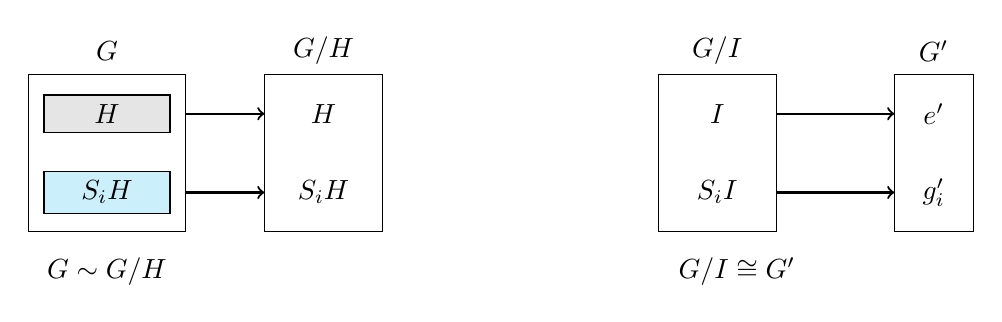
\begin{tikzpicture}
			% G ~ G/H diagram
			\begin{scope}[xshift=-4cm]
				\node at (0, -2) {$G \sim G/H$};
				\draw (-1, 0.5) rectangle (1, -1.5);
				\node at (0, 0.8) {$G$};
				\node[fill=gray!20, draw, minimum width=1.6cm] at (0, 0) {$H$};
				\node[fill=cyan!20, draw, minimum width=1.6cm] at (0, -1) {$S_i H$};

				\draw (2, 0.5) rectangle (3.5, -1.5);
				\node at (2.75, 0.8) {$G/H$};
				\node at (2.75, 0) {$H$};
				\node at (2.75, -1) {$S_i H$};

				\draw[->, thick] (1, 0) -- (2, 0);
				\draw[->, thick] (1, -1) -- (2, -1);
			\end{scope}

			% G/I ~ G' diagram
			\begin{scope}[xshift=4cm]
				\node at (0, -2) {$G/I \cong G'$};
				\draw (-1, 0.5) rectangle (0.5, -1.5);
				\node at (-0.25, 0.8) {$G/I$};
				\node at (-0.25, 0) {$I$};
				\node at (-0.25, -1) {$S_i I$};

				\draw (2, 0.5) rectangle (3, -1.5);
				\node at (2.5, 0.8) {$G'$};
				\node at (2.5, 0) {$e'$};
				\node at (2.5, -1) {$g_i'$};

				\draw[->, thick] (0.5, 0) -- (2, 0);
				\draw[->, thick] (0.5, -1) -- (2, -1);
			\end{scope}
		\end{tikzpicture}
	\end{center}
	\begin{equation}
		G \sim G', \implies G' \cong G/I 
	\end{equation}
  这表明，虽然同态的定义好像只建立了一个对应关系和乘法，似乎含有的信息非常少

  但其实，同态也蕴含了丰富的信息！如果我们把同态核 $I$ 和 $S_iI$ 都看成圈圈，那么每个圈圈中的个数都是相同的！

  也就是说，如果同态核 $I$ 中只有一个元素，那么别的圈圈（也就是陪集 $S_iI$）中也只有一个元素，这就是一对一，也就是同构，或者说非忠实表示

  如果同态核 $I$ 中有多个元素，那么别的圈圈（也就是陪集 $S_iI$）中也有多个元素，这是多对一，也就是同态，或者说非忠实表示

  于是，我们只用考察同态核的个数就能判断是否是忠实表示：

  假设 $D(G)$ 是群 $G$ 的一个表示，即 $G\sim D(G)$ ，考察群 $G$ 的同态核 $I$

  \begin{itemize}
    

    \item 如果同态核 $I$ 只有一个元素，则 $D(G)$ 是群 $G$ 的忠实表示
    \item 如果同态核 $I$ 有多个元素，则 $D(G)$ 是群 $G$ 的非忠实表示
  \end{itemize}
\end{theorem}

\begin{proof}
    对于群同态 $D: G \to GL(m, \mathbb{C})$，它是\textbf{单射}当且仅当其核 $\ker D = \{e\}$。这是一条基础结论：若 $D(g)=E$ 蕴含 $g=e$，则不同群元不可能映到同一矩阵；反之，若存在 $g\ne e$ 使 $D(g)=E$，则 $g$ 与 $e$ 有相同像，故不是单射。

    将此用于表示 $D(G)$：
    \begin{enumerate}
        \item 若 $\ker D=\{e\}$，同态 $D$ 单射，像群 $D(G)$ 与 $G$ \textbf{同构}，表示是\textbf{忠实}的。
        \item 若 $\ker D\supsetneqq\{e\}$，则存在不同群元映到同一矩阵（多对一），表示\textbf{非忠实}。依第一同构定理，还有 $D(G)\cong G/\ker D$。
    \end{enumerate}
    因而“是否忠实”与“核是否平庸”完全等价，命题得证。
\end{proof}


\subsection{群的表示举例}
一个群通常拥有无穷多个不同的表示。除了前面提到的平庸表示外，还有一类非常自然的表示。

\begin{example}{自身表示 (Defining Representation)}
    对于一个本身就是由矩阵构成的群（例如 $SO(3)$, $SU(2)$ 等），最简单、最自然的一种表示，就是把它自己作为自己的表示。
    
    也就是说，映射 D 把每一个矩阵群元 $g$ 映射到它自身：
    $$
        D(g) = g
    $$
    这个表示显然是忠实的，通常被称为该矩阵群的\textbf{自身表示}、\textbf{定义表示}或\textbf{基本表示 (Fundamental Representation)}。
\end{example}



\begin{definition}{特征标 (Character)}
    对于 $m \times m$ 的方阵 $A$，其迹 (Trace) 定义为对角元之和：
    \begin{equation}
        \text{Tr } A = \sum_{j=1}^m A_{jj}
    \end{equation}
    对于群 G 的线性表示 $G \sim D(G)$，我们将群元 $g_i$ 对应的表示矩阵 $D(g_i)$ 的迹记为 $\chi(g_i)$，并称之为该表示的\textbf{特征标}。
    \begin{equation}
        \chi(g_i) = \sum_{j=1}^m [D(g_i)]_{jj} = \text{Tr } D(g_i)
    \end{equation}
    特征标是一个标量，它描述了表示的重要特性。
\end{definition}

\begin{definition}{幺正表示与正交表示}
    \begin{itemize}
        \item 若对于群 G 中任意元素 $g_i$，其表示矩阵 $D(g_i)$ 满足 $D(g_i)^\dagger D(g_i) = E$（即 $D(g_i)$ 为幺正矩阵），则称此表示为\textbf{幺正表示 (Unitary Representation)}。
        \item 若对于群 G 中任意元素 $g_i$，其表示矩阵 $D(g_i)$ 满足 $D(g_i)^T D(g_i) = E$（即 $D(g_i)$ 为正交矩阵），则称此表示为\textbf{正交表示 (Orthogonal Representation)}。
    \end{itemize}
\end{definition}

\subsection{线性表示的性质}
\begin{property}{线性表示的基本性质}
    设 $D(G)$ 是群 G 的一个线性表示，则它满足以下性质：
    \begin{enumerate}
        \item \textbf{恒元的表示矩阵是单位矩阵}：
        \begin{equation}
            D(e) = E
        \end{equation}
        \textbf{证明}：由群公理，对于任意 $g \in G$，有 $eg = g$。根据同态性质 $D(e)D(g) = D(eg) = D(g)$。由于 $D(g)$ 是非奇异矩阵，右乘 $D(g)^{-1}$ 即得 $D(e) = E$。
        
        \item \textbf{同态关系}：
        \begin{equation}
            D(g_i)D(g_j) = D(g_i g_j)
        \end{equation}
        这是线性表示定义的直接推论。由同态定义 $G \sim D(G)$：
        \begin{equation}
            \begin{aligned}
                g_i &\to D(g_i) \\
                g_j &\to D(g_j) \\
                g_i g_j &\to D(g_i g_j)
            \end{aligned}
            \quad \implies \quad D(g_i)D(g_j) = D(g_i g_j)
        \end{equation}
        
        \item \textbf{逆元的表示矩阵是表示矩阵的逆}：
        \begin{equation}
            D(g_i^{-1}) = [D(g_i)]^{-1}
        \end{equation}
        \textbf{证明}：
        由 $g_i \to D(g_i)$ 和 $g_i^{-1} \to D(g_i^{-1})$。
        考虑到 $g_i g_i^{-1} = e$，两边取表示：
        \begin{equation}
            D(g_i g_i^{-1}) = D(g_i)D(g_i^{-1}) = D(e) = E
        \end{equation}
        由矩阵逆的定义，即得 $D(g_i)^{-1} = D(g_i^{-1})$。
    \end{enumerate}
\end{property}

\subsection{等价表示}
我们知道，线性代数中相似矩阵描述的是同一个线性变换在不同基底下的形式。这一概念也可以推广到群的表示理论中。

\begin{definition}{等价表示 (Equivalent Representation)}
    设 $D(G)$ 是群 G 的一个 m 维线性表示，设 X 是一个 $m \times m$ 的非奇异矩阵 ($\det X \neq 0$)。构造一个新的矩阵集合：
    \begin{equation}
        \bar{D}(G) = \{ \bar{D}(g_i) = X^{-1} D(g_i) X \mid g_i \in G \}
    \end{equation}
    则 $\bar{D}(G)$ 也是一个群，且 $D(G) \cong \bar{D}(G)$。我们称 $\bar{D}(G)$ 和 $D(G)$ 为群 G 的\textbf{等价表示} (或称两表示等价)。
\end{definition}

\begin{proof}[证明 $\bar{D}(G)$ 是一个群]
    $\bar{D}(G)$ 是矩阵集合，其乘法定义为矩阵乘法。
    \begin{enumerate}
        \item \textbf{存在恒元}：取 $D(e) = E$，则
        \begin{equation}
            \bar{D}(e) = X^{-1} D(e) X = X^{-1} E X = E
        \end{equation}
        显然 $E \in \bar{D}(G)$。
        \item \textbf{封闭性}：
        \begin{equation}
             \bar{D}(g_i)\bar{D}(g_j) = (X^{-1}D(g_i)X)(X^{-1}D(g_j)X) = X^{-1}D(g_i)D(g_j)X = X^{-1}D(g_i g_j)X = \bar{D}(g_i g_j) \in \bar{D}(G)
        \end{equation}
        \item \textbf{存在逆元}：
        \begin{equation}
            [\bar{D}(g_i)]^{-1} = (X^{-1} D(g_i) X)^{-1} = X^{-1} D(g_i)^{-1} X = X^{-1} D(g_i^{-1}) X = \bar{D}(g_i^{-1}) \in \bar{D}(G)
        \end{equation}
        \item \textbf{结合律}：矩阵乘法天然满足结合律。
    \end{enumerate}
    综上，$\bar{D}(G)$ 构成一个群。
\end{proof}

\begin{proof}[证明 $D(G) \cong \bar{D}(G)$ (同构)]
    \begin{enumerate}
        \item \textbf{先证同态} $D(G) \sim \bar{D}(G)$：
        定义对应关系 $D(g_i) \to \bar{D}(g_i) = X^{-1}D(g_i)X$。
        对于乘法运算，原像乘积对应 $D(g_i)D(g_j) \to \overline{D(g_i)D(g_j)} = X^{-1} D(g_i) D(g_j) X$。
        像的乘积为 $\bar{D}(g_i)\bar{D}(g_j) = X^{-1}D(g_i)XX^{-1}D(g_j)X = X^{-1}D(g_i)D(g_j)X$。
        两者相等，故保持乘法结构，即 $D(G) \sim \bar{D}(G)$。

        \item \textbf{再证同构} (即证明该映射是一一对应的)：
        多对一还是对应取决于是否存在不同的 $D(g_i)$ 映射到了同一个 $\bar{D}(g_i)$。
        反证法：假设存在 $D(g_i) \neq D(g_j)$，但对应到了同一个像 $\bar{D}(g_i) = \bar{D}(g_j)$。
        \begin{equation}
            X^{-1}D(g_i)X = X^{-1}D(g_j)X
        \end{equation}
        两边左乘 $X$ 右乘 $X^{-1}$，得：
        \begin{equation}
            X(X^{-1}D(g_i)X)X^{-1} = X(X^{-1}D(g_j)X)X^{-1} \implies D(g_i) = D(g_j)
        \end{equation}
        这与假设 $D(g_i) \neq D(g_j)$ 矛盾。
        故映射必须是一对一的。因此 $D(G) \cong \bar{D}(G)$。
    \end{enumerate}
\end{proof}

\begin{note}{等价与同构的区别}
    \begin{itemize}
        \item \textbf{等价 $\implies$ 同构}：若两表示等价，则它们的表示群同构。
        \item \textbf{等价 $\implies$ 维数相同}：相似变换不改变矩阵维数。
        \item \textbf{同构 $\not\implies$ 等价}：即使两个表示群同构且维数相同，它们也不一定等价。
    \end{itemize}

    \textbf{反例}：考虑群 $\{e, a\}$ ($a^2=e$)。
    \begin{itemize}
        \item 表示 1: $D_1(e) = [1], D_1(a) = [-1]$。
        \item 表示 2: $D_2(e) = \begin{bmatrix} 1 & 0 \\ 0 & 1 \end{bmatrix}, D_2(a) = \begin{bmatrix} 1 & 0 \\ 0 & -1 \end{bmatrix}$。
    \end{itemize}
    这两个表示群同构（但维数不同），显然不等价。

    \textbf{反例}：考虑循环群 $C_3 = \{1, a, a^2\}$，令 $\omega = e^{2\pi i / 3},\omega^{3}=1$。
    \begin{itemize}
        \item 表示 1: $\rho_1(1) = 1, \rho_1(a) = \omega$,所以 $\rho_1(a^{2}) = \omega^{2}$
        \item 表示 2: $\rho_2(1) = 1, \rho_2(a) = \omega^2$,所以 $\rho_1(a^{2}) = \omega^{4}=\omega$
    \end{itemize}
    这两个表示维数相同（均为 1），且像作为群是同构的（均为 $\{1, \omega, \omega^2\}$），但由于 $\rho_1(a) \neq \rho_2(a)$，它们显然不等价。
    
    \textbf{严格判据}：
    设 $D(G), \bar{D}(G)$ 为群 G 的两个\textbf{维数相同}的表示。若\textbf{存在}矩阵 X 且 $\det X \neq 0$，使得：
    \begin{equation}
        \forall g_i \in G, \quad \bar{D}(g_i) = X^{-1} D(g_i) X
    \end{equation}
    则称 $\bar{D}(G)$ 与 $D(G)$ 等价。注意：只有扫遍所有可能的 X 都无法满足时，才称不等价。如果你只是拿了一个 $X$ 算过后发现不能对角化，这并不能证明不等价
\end{note}

\begin{property}{等价的传递性}
    两表示维度相同，且等价于同一相同维度的表示，则此两表示等价。
\end{property}

% 到这里，你会发现判断是否可约，似乎只能通过看表示矩阵 $D(g_{i} )$ 是否可对角化来判断，到后面我们会介绍用特征标的更方便的方法

% 现在，只能通过判断可对角化来判断是否可约，我们会介绍

\subsection{可约与不可约表示}
\begin{definition}{可约表示 (Reducible Representation)}
    设 $D(G)$ 是群 G 的一个 m 维表示。若\textbf{存在}非奇异矩阵 X ($\det X \neq 0$)，使得对 G 中\textbf{每一个}元素 $g$，变换后的矩阵 $\bar{D}(g) = X^{-1}D(g)X$ 都具有相同的\textbf{上三角形}或\textbf{下三角形}的分块形式：
    
    \textbf{形式一（上三角分块）}：
    \begin{equation}
        \bar{D}(g) = \begin{bmatrix} D_1(g) & M(g) \\ 0 & D_2(g) \end{bmatrix}
    \end{equation}
    
    \textbf{形式二（下三角分块）}：
    \begin{equation}
        \bar{D}(g) = \begin{bmatrix} D_1(g) & 0 \\ M(g) & D_2(g) \end{bmatrix}
    \end{equation}
    其中 $D_1(g)$ 是 $k \times k$ 矩阵，$D_2(g)$ 是 $l \times l$ 矩阵 ($k+l=m$)，且 $0$ 代表全零子块。
    
    满足上述条件的表示 $D(G)$ 称为群 G 的一个\textbf{可约表示}。
    反之，若找不到这样的矩阵 X 将表示矩阵同时化为分块三角形式，则称该表示为\textbf{不可约表示 (Irreducible Representation)}。
\end{definition}

\begin{note}{对可约性的理解}
    \begin{itemize}
        \item In other words，可约就是可化约， $\bar{D}(G)$ 可以化为块状上三角或块状下三角。
        \item 对角元上的每一块称为\textbf{准对角元}。
        \item \textbf{一维表示的不可约性}：显然，一维表示是 $1 \times 1$ 矩阵，不可能再进行分块拆分，因此\textbf{一维表示一定是不可约的}。
        \item \textbf{等价性保持}：可约表示的等价表示依然是可约的；不可约表示的等价表示依然是不可约的。
    \end{itemize}
\end{note}

\subsection{准对角元构成群表示}
在讨论可约表示时，我们发现将表示矩阵化为上三角（或下三角）形式后，其对角线上的子块具有特殊的性质。

\begin{theorem}{准对角元构成群表示}{quasi_diag_is_rep}
    设 $D(G)$ 是群 $G$ 的一个可约表示，且已被化为上三角分块形式：
    \begin{equation}
        \forall g \in G, \quad \bar{D}(g) = \begin{bmatrix} D_1(g) & M(g) \\ 0 & D_2(g) \end{bmatrix}
    \end{equation}
    其中 $D_1(g)$ 和 $D_2(g)$ 是位于对角线上的方阵，称为\textbf{准对角元} (Quasi-diagonal elements)。
    
    \textbf{结论}：$D_1(G) = \{D_1(g) \mid g \in G\}$ 和 $D_2(G) = \{D_2(g) \mid g \in G\}$ 自身也构成群，并且分别是群 $G$ 的表示。
\end{theorem}

\begin{proof}
    由群表示的定义，我们只需要证明这些准对角元集合保持了群 $G$ 的乘法结构（即同态性）。
    
    \begin{enumerate}
        \item \textbf{考察原表示的乘法关系}：
    对于群中任意两个元素 $g_i, g_j \in G$，根据表示的同态性质，有：
    \begin{equation}
        \bar{D}(g_i g_j) = \bar{D}(g_i) \bar{D}(g_j)
    \end{equation}
    
        \item \textbf{展开矩阵乘法}：
    将分块矩阵代入等式右边：
    \begin{equation}
        \begin{aligned}
            \bar{D}(g_i) \bar{D}(g_j) &= \begin{bmatrix} D_1(g_i) & M(g_i) \\ 0 & D_2(g_i) \end{bmatrix} \begin{bmatrix} D_1(g_j) & M(g_j) \\ 0 & D_2(g_j) \end{bmatrix} \\
            &= \begin{bmatrix} D_1(g_i)D_1(g_j) & D_1(g_i)M(g_j) + M(g_i)D_2(g_j) \\ 0 & D_2(g_i)D_2(g_j) \end{bmatrix}
        \end{aligned}
    \end{equation}
    
        \item \textbf{比较对应元素}：
    等式左边的 $\bar{D}(g_i g_j)$ 根据定义写作：
    \begin{equation}
        \bar{D}(g_i g_j) = \begin{bmatrix} D_1(g_i g_j) & M(g_i g_j) \\ 0 & D_2(g_i g_j) \end{bmatrix}
    \end{equation}
    比较两端矩阵的对应分块，特别是对角线上的子块，我们得到：
    \begin{equation}
        \begin{aligned}
            D_1(g_i g_j) &= D_1(g_i) D_1(g_j) \\
            D_2(g_i g_j) &= D_2(g_i) D_2(g_j)
        \end{aligned}
    \end{equation}
    
        \item \textbf{结论}：
        这表明映射 $g \to D_1(g)$ 和 $g \to D_2(g)$ 均满足同态条件 $D(ab) = D(a)D(b)$。此外，由于 $D(e) = E$，显然 $D_1(e)$ 和 $D_2(e)$ 也是单位矩阵。因此，$D_1(G)$ 和 $D_2(G)$ 都是群 $G$ 的合法线性表示。
    \end{enumerate}
\end{proof}

\subsection{可约表示的约化}
既然准对角元 $D_1(G)$ 也是 $G$ 的一个表示，我们自然可以问：$D_1(G)$ 是否可约？
如果 $D_1(G)$ 仍然是可约的，我们可以对它再次进行相似变换，将其进一步拆解。对 $D_2(G)$ 亦然。

这个过程可以一直进行下去，直到对角线上所有的子块都\textbf{不能再约化}（即成为不可约表示）为止。这个过程称为\textbf{可约表示的约化}。

最终，我们将得到一个分块上三角矩阵，其对角元全部由不可约表示组成：
\begin{equation}
    \bar{D}(G) \sim \begin{bmatrix} 
        \tilde{D}_1(G) & \dots & \dots \\
         0 & \tilde{D}_2(G) & \dots \\
         \vdots & \ddots & \ddots \\
         0 & \dots & \tilde{D}_k(G)
    \end{bmatrix}
\end{equation}
其中 $\tilde{D}_i(G)$ 为不可约表示。需要注意的是，分解出的这些不可约表示中，可能存在相同或等价的表示。

\subsection{完全可约表示与直和分解}
\begin{definition}{完全可约表示 (Fully Reducible)}
    若存在非奇异矩阵 $X$，使得群 $G$ 的表示 $D(G)$ 可以被对角化为\textbf{分块对角矩阵}（即除了准对角元外，其余位置全为 $0$）：
    \begin{equation}
        X^{-1}D(g)X = \begin{bmatrix} 
            \tilde{D}_1(g) & 0 & \dots & 0 \\
            0 & \tilde{D}_2(g) & \dots & 0 \\
            \vdots & \vdots & \ddots & \vdots \\
            0 & 0 & \dots & \tilde{D}_k(g)
        \end{bmatrix}
    \end{equation}
    则称该表示为\textbf{完全可约表示}。
\end{definition}

\begin{note}
    \textbf{有限群的性质}：对于有限群，任何可约表示都一定是完全可约的（Maschke 定理）。这意味着对于有限群，我们总能把右上角的 $M(g)$ 部分消除掉。但对于连续群（如平移群），则不一定。
\end{note}

\subsubsection{直和分解 (Direct Sum)}
为了简洁地描述完全可约表示的结构，我们引入\textbf{直和}的概念。
设群 $G$ 共有 $r$ 个不等价的不可约表示，记为 $\tilde{D}_1(G), \tilde{D}_2(G), \dots, \tilde{D}_r(G)$。

任意一个完全可约表示 $D(G)$ 分解后，可能会包含 $n_1$ 个 $\tilde{D}_1$， $n_2$ 个 $\tilde{D}_2$ 等等。我们可以通过排列行和列，将相同的不可约表示归并在一起。
形象地，约化后的矩阵结构如下所示：

\begin{equation}
    X^{-1}D(G)X = \left[
    \begin{array}{c|c|c|c}
        \underbrace{\begin{matrix} \tilde{D}_1 & & \\ & \ddots & \\ & & \tilde{D}_1 \end{matrix}}_{n_1 \text{个}} & 0 & \dots & 0 \\
        \hline
        0 & \underbrace{\begin{matrix} \tilde{D}_2 & & \\ & \ddots & \\ & & \tilde{D}_2 \end{matrix}}_{n_2 \text{个}} & \dots & 0 \\
        \hline
        \vdots & \vdots & \ddots & \vdots \\
        \hline
        0 & 0 & \dots & \underbrace{\begin{matrix} \tilde{D}_r & & \\ & \ddots & \\ & & \tilde{D}_r \end{matrix}}_{n_r \text{个}}
    \end{array}
    \right]
\end{equation}

数学上，记作\textbf{直和}形式：
\begin{equation}
    D(G) \cong n_1 \tilde{D}_1(G) \oplus n_2 \tilde{D}_2(G) \oplus \dots \oplus n_r \tilde{D}_r(G) = \bigoplus_{k=1}^r n_k \tilde{D}_k(G)
\end{equation}
其中 $n_k$ 称为不可约表示 $\tilde{D}_k$ 在 $D$ 中出现的\textbf{次数} (Multiplicity)。

\section{群表示举例}

\begin{example}{Eg.1: SO(2) 的表示}
    $SO(2)$ 群由二维平面上保持长度的旋转构成，群元可以用旋转角 $\phi \in [0, 2\pi)$ 参数化。
    
    \begin{enumerate}
        \item \textbf{一维表示与忠实性讨论}
    一般形式的一维表示为：
    \begin{equation}
        D^{(n)}(\phi) = e^{in\phi}, \quad n \in \mathbb{Z}
    \end{equation}
    \textbf{问题}：什么样的 $n$ 使得它是忠实（真实）表示？
    根据定理 \ref{thm:the-ifTruthful} ，只用考察同态核的元素个数即可

    \textbf{分析}：考察同态核 $K = \{ \phi \in [0, 2\pi) \mid D^{(n)}(\phi) = 1 \}$。
    \begin{equation}
        e^{in\phi} = 1 \implies n\phi = 2k\pi \quad (k \in \mathbb{Z})
    \end{equation}
    \begin{itemize}
        \item 若 $n=0$，则 $D(\phi) \equiv 1$。所有 $\phi$ 都在核内，核非平庸，\textbf{非忠实}（平庸表示）。
        \item 若 $n=1$，则 $\phi = 2k\pi$。在 $[0, 2\pi)$ 区间内仅有 $\phi=0$。核 $K=\{e\}$，\textbf{忠实表示}。
        \item 若 $n=-1$，同理，核 $K=\{e\}$，\textbf{忠实表示}。
        \item 若 $|n| \ge 2$，例如 $n=2$。则 $\phi = 0$ 或 $\phi = \pi$ 时，$e^{i2\phi}=1$。此时核 $K=\{0, \pi\} \neq \{e\}$。这表示群中两个不同的元素映射到了同一个矩阵数值 1。这是一个“二对一”的同态。因此，\textbf{非忠实}。
    \end{itemize}
    \textbf{结论}：对于 $SO(2)$ 群，$D^{(n)}(\phi)$ 仅当 $n = \pm 1$ 时为忠实表示。当 $|n| \ge 2$ 时，它是非忠实的（实际上是商群 $SO(2)/C_n$ 的表示）。

        \item \textbf{三维表示}
    我们可以通过将二维旋转扩充到三维空间（绕某一轴旋转）来构造三维表示。这些表示显然是可约的（由 $2 \times 2$ 旋转块和 $1$ 组成）。
    \begin{itemize}
        \item \textbf{绕 z 轴旋转} ($R_z$):
        \begin{equation}
            D_z(\phi) = \begin{bmatrix} \cos\phi & -\sin\phi & 0 \\ \sin\phi & \cos\phi & 0 \\ 0 & 0 & 1 \end{bmatrix} = D^{(2D)}(\phi) \oplus 1
        \end{equation}
        \item \textbf{绕 x 轴旋转} ($R_x$):
        \begin{equation}
            D_x(\phi) = \begin{bmatrix} 1 & 0 & 0 \\ 0 & \cos\phi & -\sin\phi \\ 0 & \sin\phi & \cos\phi \end{bmatrix} = 1 \oplus D^{(2D)}(\phi)
        \end{equation}
        \item \textbf{绕 y 轴旋转} ($R_y$):
        \begin{equation}
            D_y(\phi) = \begin{bmatrix} \cos\phi & 0 & \sin\phi \\ 0 & 1 & 0 \\ -\sin\phi & 0 & \cos\phi \end{bmatrix}
        \end{equation}
        注意 $R_y$ 的形式虽然看起来像插空，但通过基底变换（交换 $y$ 和 $z$ 轴）也可以化为直和形式。
    \end{itemize}
        \end{enumerate}
\end{example}

\begin{example}{Eg.2: 平移群 T(a) 的表示}
    (此处略去详细推导，参考前文，重点在于 $e^{ca}$ 的实虚分类以及 Jordan 块构成的非完全可约表示。)
\end{example}

\begin{example}{Eg.3: n 阶循环群 $C_n$ 的表示}
    $C_n = \{a, a^2, \dots, a^n=e\}$。我们可以将其视为平面上对正 $n$ 边形的旋转对称操作。
    
    \begin{enumerate}
        \item \textbf{n 维表示 (坐标轮换)}
    考虑圆周上均匀分布的 $n$ 个点（或 $n$ 个基向量），标记为 $1, 2, \dots, n$。
    % [示意图描述：一个圆周，顺时针或逆时针标记点 1 到 n。群元 a 使得点 1->2, 2->3, ..., n->1]
    群元 $a$ 的作用是将每个位置上的坐标“推”向下一个位置。
    即：$p_1 \to p_2, p_2 \to p_3, \dots, p_n \to p_1$。
    写成矩阵形式：
    \begin{equation}
        \begin{bmatrix} p_2 \\ p_3 \\ \vdots \\ p_n \\ p_1 \end{bmatrix} = 
        \begin{bmatrix} 
            0 & 1 & 0 & \dots & 0 \\
            0 & 0 & 1 & \dots & 0 \\
            \vdots & \vdots & \ddots & \ddots & \vdots \\
            0 & 0 & 0 & \dots & 1 \\
            1 & 0 & 0 & \dots & 0
        \end{bmatrix}
        \begin{bmatrix} p_1 \\ p_2 \\ \vdots \\ p_{n-1} \\ p_n \end{bmatrix}
    \end{equation}
    我们记这个矩阵为 $\bar{D}_1(a)$。显然，这是一个 $n \times n$ 的置换矩阵。
    
    对于群中的其他元素 $a^2$（移动 2 步），$a^k$（移动 k 步）：
    \begin{equation}
        \bar{D}_1(a^k) = [\bar{D}_1(a)]^k
    \end{equation}
    例如，对于 $a^2$，矩阵形式中 $1$ 的位置会向右移两格。
    这构成了一个 $n$ 维表示，记为 $\bar{D}_{reg}(C_n)$ (正则表示)。它是\textbf{可约}的。

        \item \textbf{一维表示与忠实性分析}
    由于 $C_n$ 是阿贝尔群，其不可约表示必然是一维的。
    设 $D(a) = \lambda$ (复数)。由 $a^n = e$，得 $\lambda^n = 1$。
    故 $\lambda$ 必须是 $1$ 的 $n$ 次单位根：
    \begin{equation}
        \lambda_k = e^{i \frac{2\pi k}{n}}, \quad k = 0, 1, \dots, n-1
    \end{equation}
    这给出了 $n$ 个不同的一维表示：
    \begin{equation}
        D_k(a^m) = e^{i \frac{2\pi k m}{n}}
    \end{equation}
    
    \textbf{忠实性讨论 (通过同态核判别)}：
    表示是忠实的 $\iff$ 同态核 $I = \{e\}$ (单射)。
    若同态核包含除 $e$ 以外的元素，说明有多个群元映射到了单位元 $1$，即“多对一”，故非忠实。
    
    考察同态核 $I_k = \{ a^m \in C_n \mid D_k(a^m) = 1 \}$：
    \begin{equation}
        e^{i \frac{2\pi k m}{n}} = 1 \implies \frac{km}{n} \in \mathbb{Z} \implies n \mid km
    \end{equation}
    其中 $1 \le m \le n$。
    \begin{itemize}
        \item \textbf{情形 1：$\gcd(k, n) = 1$ (k 与 n 互质)}
        若 $n$ 与 $k$ 互质，要使 $n \mid km$，必须有 $n \mid m$。在 $1 \le m \le n$ 范围内，只有 $m=n$（即 $a^n=e$）。
        故核 $I_k = \{e\}$。同态是“一对一”的。
        $\implies$ \textbf{忠实表示}。
        
        \item \textbf{情形 2：$\gcd(k, n) = d > 1$}
        此时 $n$ 和 $k$ 有公因子 $d$。取 $m = n/d$。显然 $m < n$ (即 $a^m \neq e$)。
        验证：$\frac{k m}{n} = \frac{k (n/d)}{n} = \frac{k}{d}$。因为 $d \mid k$，所以 $k/d$ 是整数，满足条件。
        故存在非恒元 $a^{n/d}$ 在核内。核 $I_k$ 非平庸。
        根据同构定理 $G/I \cong D(G)$，这是一个“$|I|$ 对 1”的同态。
        $\implies$ \textbf{非忠实表示}。
    \end{itemize}
    
    \textbf{特别例子}：
    \begin{itemize}
        \item $k=0$: $D_0(a)=1$。核为 $C_n$ 全体。平庸表示，非忠实。
        \item $k=1$: $\gcd(1, n)=1$。忠实表示。
        \item 设 $n=4, k=2$: $\gcd(4,2)=2 \neq 1$。$D_2(a) = e^{i\pi} = -1$, $D_2(a^2) = 1$。核包含 $a^2$。非忠实。
    \end{itemize}

        \item \textbf{总结}
    我们实际上通过 $k=0, 1, \dots, n-1$ 找到了 $C_n$ 群的\textbf{所有 $n$ 个不等价的不可约表示}。
    \begin{itemize}
        \item $D_k(C_n)$ 是不可约的（一维）。
        \item 当 $\gcd(k, n)=1$ 时，是忠实表示。
        \item 之前的 $n$ 维坐标轮换表示 $\bar{D}_1$ 是可约的，它可以完全约化为这 $n$ 个一维表示的直和：
        \begin{equation}
            \bar{D}_1(C_n) \cong D_0(C_n) \oplus D_1(C_n) \oplus \dots \oplus D_{n-1}(C_n)
        \end{equation}
    \end{itemize}
        \end{enumerate}
\end{example}


\section{群表示举例}

\begin{example}{Eg.1: SO(2) 的表示}
    $SO(2)$ 群由二维平面上保持长度的旋转构成，群元可以用旋转角 $\phi \in [0, 2\pi)$ 参数化。
    
    \begin{enumerate}
        \item \textbf{一维表示与忠实性讨论}
    一般形式的一维表示为：
    \begin{equation}
        D^{(n)}(\phi) = e^{in\phi}, \quad n \in \mathbb{Z}
    \end{equation}
    \textbf{问题}：什么样的 $n$ 使得它是忠实（真实）表示？
    根据定理 \ref{thm:the-ifTruthful} ，只用考察同态核的元素个数即可

    \textbf{分析}：考察同态核 $K = \{ \phi \in [0, 2\pi) \mid D^{(n)}(\phi) = 1 \}$。
    \begin{equation}
        e^{in\phi} = 1 \implies n\phi = 2k\pi \quad (k \in \mathbb{Z})
    \end{equation}
    \begin{itemize}
        \item 若 $n=0$，则 $D(\phi) \equiv 1$。所有 $\phi$ 都在核内，核非平庸，\textbf{非忠实}（平庸表示）。
        \item 若 $n=1$，则 $\phi = 2k\pi$。在 $[0, 2\pi)$ 区间内仅有 $\phi=0$。核 $K=\{e\}$，\textbf{忠实表示}。
        \item 若 $n=-1$，同理，核 $K=\{e\}$，\textbf{忠实表示}。
        \item 若 $|n| \ge 2$，例如 $n=2$。则 $\phi = 0$ 或 $\phi = \pi$ 时，$e^{i2\phi}=1$。此时核 $K=\{0, \pi\} \neq \{e\}$。这表示群中两个不同的元素映射到了同一个矩阵数值 1。这是一个“二对一”的同态。因此，\textbf{非忠实}。
    \end{itemize}
    \textbf{结论}：对于 $SO(2)$ 群，$D^{(n)}(\phi)$ 仅当 $n = \pm 1$ 时为忠实表示。当 $|n| \ge 2$ 时，它是非忠实的（实际上是商群 $SO(2)/C_n$ 的表示）。

        \item \textbf{二维表示}
    \begin{equation}
        D_2(\phi) = \begin{bmatrix} \cos\phi & -\sin\phi \\ \sin\phi & \cos\phi \end{bmatrix}
    \end{equation}
    这是一个\textbf{可约表示}，它是可对角化的。通过复数基底变换可以化为对角形：
    \begin{equation}
        X^{-1}D_2(\phi)X = \begin{bmatrix} e^{i\phi} & 0 \\ 0 & e^{-i\phi} \end{bmatrix} = e^{i\phi} \oplus e^{-i\phi}
    \end{equation}

        \item \textbf{三维表示}
    我们可以通过将二维旋转扩充到三维空间（绕某一轴旋转）来构造三维表示。这些表示显然是可约的（由 $2 \times 2$ 旋转块和 $1$ 组成）。
    \begin{itemize}
        \item \textbf{绕 z 轴旋转} ($R_z$):
        \begin{equation}
            D_z(\phi) = \begin{bmatrix} \cos\phi & -\sin\phi & 0 \\ \sin\phi & \cos\phi & 0 \\ 0 & 0 & 1 \end{bmatrix} = D_2(\phi) \oplus 1
        \end{equation}
        \item \textbf{绕 x 轴旋转} ($R_x$):
        \begin{equation}
            D_x(\phi) = \begin{bmatrix} 1 & 0 & 0 \\ 0 & \cos\phi & -\sin\phi \\ 0 & \sin\phi & \cos\phi \end{bmatrix} = 1 \oplus D_2(\phi)
        \end{equation}
        \item \textbf{绕 y 轴旋转} ($R_y$):
        \begin{equation}
            D_y(\phi) = \begin{bmatrix} \cos\phi & 0 & \sin\phi \\ 0 & 1 & 0 \\ -\sin\phi & 0 & \cos\phi \end{bmatrix}
        \end{equation}
        注意 $R_y$ 的形式虽然看起来像插空，但通过基底变换（交换 $y$ 和 $z$ 轴）也可以化为直和形式。
    \end{itemize}
    
        \end{enumerate}
    \textbf{推广}：对于任意 $n$ 维，我们可以构造如下的可约表示：
    \begin{equation}
        1 \oplus e^{i\phi} \oplus e^{i3\phi} = \begin{bmatrix} 1 & & \\ & e^{i\phi} & \\ & & e^{i3\phi} \end{bmatrix}
    \end{equation}
    或者：
    \begin{equation}
        e^{i\phi} \oplus \begin{bmatrix} \cos n\phi & -\sin n\phi \\ \sin n\phi & \cos n\phi \end{bmatrix} = \begin{bmatrix} e^{i\phi} & 0 & 0 \\ 0 & \cos n\phi & -\sin n\phi \\ 0 & \sin n\phi & \cos n\phi \end{bmatrix}
    \end{equation}
\end{example}

\begin{example}{Eg.2: 平移群 T(a) 的表示}
    平移群满足 $T(a)T(b) = T(a+b)$。

    \begin{enumerate}
        \item \textbf{一维表示}
    \begin{itemize}
        \item \textbf{平庸表示}：$D_1(a) = 1$。
        \item \textbf{一般表示}：$D_2(a) = e^a$ 或 $D_2(a) = e^{ca}$。
        验证同态性：$D(a)D(b) = e^{ca}e^{cb} = e^{c(a+b)} = D(a+b)$。
        \begin{itemize}
            \item 若 $c$ 为纯虚数，则具有周期性非平凡（如晶格中的 Bloch 波）。
            \item 若 $c \in \mathbb{R}$，则为实表示。
        \end{itemize}
        \item \textbf{思考}：$D_4 = e^{a+ia}$ 是真实表示吗？
    \end{itemize}

        \item \textbf{二维表示 (Jordan 块)}
    \begin{equation}
        D_5(a) = \begin{bmatrix} 1 & a \\ 0 & 1 \end{bmatrix}
    \end{equation}
    验证同态性：
    \begin{equation}
        \begin{bmatrix} 1 & a \\ 0 & 1 \end{bmatrix} \begin{bmatrix} 1 & x \\ 0 & 1 \end{bmatrix} = \begin{bmatrix} 1 & x+a \\ 0 & 1 \end{bmatrix} = D_5(a+x)
    \end{equation}
    这是一个\textbf{可约表示}（因为它是上三角矩阵），但是它是\textbf{不完全可约表示}（Not fully reducible）。因为它已经是 Jordan 标准型，无法通过相似变换对角化。
    这也是一个\textbf{真实表示}（忠实表示）。

        \item \textbf{n 维表示}
    \begin{equation}
        D_6(a) = \begin{bmatrix} 
            1 & a & & & \\ 
             & 1 & a & & \\ 
             & & \ddots & \ddots & \\ 
             & & & 1 & a \\ 
             & & & & 1 
        \end{bmatrix}
    \end{equation}
    \end{enumerate}
\end{example}

\begin{example}{Eg.3: n 阶循环群 $C_n$ 的表示}
    $C_n = \{a, a^2, \dots, a^n=e\}$。群元可以当作二维平面上的转动。

    \begin{enumerate}
        \item \textbf{一维表示}
    \begin{itemize}
        \item $D_0(a) = 1$：平庸表示，恒等表示。
        \item $D_1(a) = e^{i\frac{2\pi}{n}}$：真实表示。
        \item 一般形式：
        \begin{equation}
            D_k(a) = e^{ik\frac{2\pi}{n}}, \quad k \in \mathbb{Z}
        \end{equation}
        若取 $n=4, k=2$，则 $D_2(a) = e^{i\pi} = -1$，但 $D_2(a^2) = (-1)^2 = 1 = D_2(e)$。此时核不为 $\{e\}$，故为\textbf{非忠实表示}。
        一般结论：当 $|k| \ge 2$ 时可能为非真实表示。
    \end{itemize}
    该群的一维表示集合为：
    \begin{equation}
        D_k(C_n) = \{ D_k(a^m) = e^{ik\frac{2\pi}{n}m} \mid m=1, 2, \dots, n \}
    \end{equation}
    \textbf{问题}：这是否也是真实表示？需考察同态核。

        \item \textbf{一维表示与忠实性分析}
    由于 $C_n$ 是阿贝尔群，其不可约表示必然是一维的。
    设 $D(a) = \lambda$ (复数)。由 $a^n = e$，得 $\lambda^n = 1$。
    故 $\lambda$ 必须是 $1$ 的 $n$ 次单位根：
    \begin{equation}
        \lambda_k = e^{i \frac{2\pi k}{n}}, \quad k = 0, 1, \dots, n-1
    \end{equation}
    这给出了 $n$ 个不同的一维表示：
    \begin{equation}
        D_k(a^m) = e^{i \frac{2\pi k m}{n}}
    \end{equation}
    
    \textbf{忠实性讨论 (通过同态核判别)}：
    表示是忠实的 $\iff$ 同态核 $I = \{e\}$ (单射)。
    若同态核包含除 $e$ 以外的元素，说明有多个群元映射到了单位元 $1$，即“多对一”，故非忠实。
    
    考察同态核 $I_k = \{ a^m \in C_n \mid D_k(a^m) = 1 \}$：
    \begin{equation}
        e^{i \frac{2\pi k m}{n}} = 1 \implies \frac{km}{n} \in \mathbb{Z} \implies n \mid km
    \end{equation}
    其中 $1 \le m \le n$。
    \begin{itemize}
        \item \textbf{情形 1：$\gcd(k, n) = 1$ (k 与 n 互质)}
        若 $n$ 与 $k$ 互质，要使 $n \mid km$，必须有 $n \mid m$。在 $1 \le m \le n$ 范围内，只有 $m=n$（即 $a^n=e$）。
        故核 $I_k = \{e\}$。同态是“一对一”的。
        $\implies$ \textbf{忠实表示}。
        
        \item \textbf{情形 2：$\gcd(k, n) = d > 1$}
        此时 $n$ 和 $k$ 有公因子 $d$。取 $m = n/d$。显然 $m < n$ (即 $a^m \neq e$)。
        验证：$\frac{k m}{n} = \frac{k (n/d)}{n} = \frac{k}{d}$。因为 $d \mid k$，所以 $k/d$ 是整数，满足条件。
        故存在非恒元 $a^{n/d}$ 在核内。核 $I_k$ 非平庸。
        根据同构定理 $G/I \cong D(G)$，这是一个“$|I|$ 对 1”的同态。
        $\implies$ \textbf{非忠实表示}。
    \end{itemize}
    
    \textbf{特别例子}：
    \begin{itemize}
        \item $k=0$: $D_0(a)=1$。核为 $C_n$ 全体。平庸表示，非忠实。
        \item $k=1$: $\gcd(1, n)=1$。忠实表示。
        \item 设 $n=4, k=2$: $\gcd(4,2)=2 \neq 1$。$D_2(a) = e^{i\pi} = -1$, $D_2(a^2) = 1$。核包含 $a^2$。非忠实。
    \end{itemize}


    \end{enumerate}
    \begin{enumerate}
        \item \textbf{n 维表示：坐标的循环}
    % [此处需要一个示意图：一个圆周上均匀分布着 n 个点，标号 1 到 n，箭头指示逆时针旋转 1->2, 2->3 ... n->1]
    考虑 $n$ 个基向量（坐标）的循环置换：
    \begin{equation}
        \begin{bmatrix} 
             & & & 1 \\ 
            1 & & & \\ 
             & \ddots & & \\ 
             & & 1 & 
        \end{bmatrix} 
        \begin{bmatrix} p_1 \\ p_2 \\ \vdots \\ p_n \end{bmatrix} 
        = 
        \begin{bmatrix} p_n \\ p_1 \\ \vdots \\ p_{n-1} \end{bmatrix}
    \end{equation}
    记此表示矩阵为 $\bar{D}_1(a)$：
    \begin{equation}
        \bar{D}_1(a) = \begin{bmatrix} 
            0 & \dots & & 1 \\ 
            1 & 0 & & \\ 
             & \ddots & \ddots & \\ 
             & & 1 & 0 
        \end{bmatrix}
    \end{equation}
    对于群中其他元素：$\bar{D}_1(a^2) = (\bar{D}_1(a))^2$。

        \item \textbf{更多的 n 维表示 (表示 K)}
    我们可以构造表示 $K$，即移动 $k$ 步的矩阵：
    \begin{equation}
        \bar{D}_k(a) = (D_1(a))^k = \begin{bmatrix} 
            0_{k \times (n-k)} & E_{k \times k} \\ 
            E_{(n-k) \times (n-k)} & 0_{(n-k) \times k} 
        \end{bmatrix}
    \end{equation}
    且有 $\bar{D}_k(a^i) = [\bar{D}_k(a)]^i$。
    这给出了 $n$ 个 $n$ 维表示。

    \end{enumerate}
    \textbf{注意：}
    \begin{enumerate}
        \item $D_k(C_n)$ (一维) 与 $\bar{D}_k(C_n)$ (n维) 同构，但\textbf{不等价}（当 $n \ge 2$ 时维数不同）。
        \item $D_k(C_n)$ 是\textbf{不可约表示}，而 $\bar{D}_k(C_n)$ 是\textbf{可约表示}。
        \item $D_1(C_n), \dots, D_n(C_n)$ 是 $C_n$ 的所有 $n$ 个不等价不可约表示。
    \end{enumerate}
\end{example}

















\section{标量函数的变换算符与表示的构造}

\subsection{标量函数}
\begin{itemize}
    \item \textbf{定义}：$\phi(x) = \phi'(x')$，即标量函数的值不随坐标的变换而改变。
    \item \textbf{用途}：标量函数用来描述标量场。
    \item $\phi$ 是空间的函数，$\phi = \phi(x)$。在空间中的每一点，$\phi(x)$ 都是标量。
    \item \textbf{例子}：温度 $T(x)$、密度 $\rho(x)$ 等。
\end{itemize}

\begin{note}
    场包括标量场、张量场、旋量场（电子的场，Fermi 子？）等。
\end{note}

\subsection{标量函数的变换算符}
对于当物理系统（标量场）发生改变时，标量函数如何变化？我们有两种理解方式：
\begin{enumerate}
    \item \textbf{主动观点 (Active View)}：系统变，坐标系不变。
    \item \textbf{被动观点 (Passive View)}：坐标系变，系统不变。
\end{enumerate}

% 
% [此处需要一个示意图：展示主动变换和被动变换的区别。图1：坐标系固定，物体（标量场）发生移动或旋转；图2：物体固定，坐标系发生移动或旋转。标注 x, x', R, \psi(x), \psi'(x') 等符号]
%

由于 $\psi'(x') = \psi(x)$，标量函数的形式不随坐标的变换而改变。

记 $R$ 为 $x$ 到 $x'$ 的变换：
\begin{equation}
    R: x \to x', \quad x' = Rx, \quad x = R^{-1}x'
\end{equation}

为了使标量函数的形式不变，则在相应的坐标变换后，\textbf{标量函数的形式也应发生相应的变换}。即由 $\psi$ 变换为 $\psi'$。显然这个变换与坐标变换 $R$ 有关，记为 $P_R$。
\begin{equation}
    P_R \psi = \psi'
\end{equation}
由于是相同形式的函数，变量相同，满足：
\begin{equation}
    P_R \psi(x) = \psi'(x)
\end{equation}

$P_R$ 是由 $R$ 诱导出的一个算符，它把变换前的标量函数 $\psi$ 变换为 $\psi'$。

推导如下：
\begin{equation}
    R: x \to x' \implies P_R: \psi \to \psi' = P_R \psi
\end{equation}
由标量性质 $\psi'(x') = \psi(x)$，代入 $x = R^{-1}x'$：
\begin{equation}
    \psi'(x') = \psi(R^{-1}x')
\end{equation}
由于 $x'$ 是任意坐标变量，我们可以将 $x'$ 替换为 $x$，得到新老函数在函数值上的联系：
\begin{equation}
    P_R \psi(x) = \psi'(x) = \psi(R^{-1}x)
\end{equation}

这也给出了 $P_R$ 对任意标量函数的变换规则：

\textbf{只要把 $\psi(x)$ 的自变量换为 $R^{-1}x$，整个函数作为 $x$ 的函数，就得到了新函数 $\psi'(x)$。}
\begin{equation}
    \psi'(x) = \psi(R^{-1}x)
\end{equation}

\begin{example}
    设 $\psi(\vec{r}) = xy$ 为标量。
    设变换 $R$ 为：$x \to -x, y \to y, z \to z$（关于 $yz$ 平面的反射）。
    则 $R^{-1}$ 为：$x \to -x, y \to y, z \to z$。
    
    应用算符 $P_R$：
    \begin{equation}
        P_R \psi(\vec{r}) = \psi'(\vec{r}) = \psi(R^{-1}\vec{r}) = \psi(-x, y) = (-x)y = -xy
    \end{equation}
\end{example}

\subsection{变换算符群与坐标变换群的同构}
\begin{theorem}{群同构}{isomorphism_PR_R}
    若 $\{R\}$ 是一个群，则 $\{P_R\}$ 也构成群，且 $\{R\}$ 与 $\{P_R\}$ 同构。
    \begin{equation}
        \{R\} \cong \{P_R\}
    \end{equation}
\end{theorem}

\begin{proof}
    \textbf{1. 先证 $P_R$ 是线性算符}
    设 $\eta(x) = a\psi(x) + b\phi(x)$。
    根据 $P_R$ 定义，有 $P_R \eta(x) = \eta(R^{-1}x)$。
    \begin{equation}
        \begin{aligned}
            P_R [a\psi(x) + b\phi(x)] &= a\psi(R^{-1}x) + b\phi(R^{-1}x) \\
            &= a P_R \psi(x) + b P_R \phi(x)
        \end{aligned}
    \end{equation}
    故 $P_R$ 是线性的。

    \textbf{2. 再证 $P_{SR} = P_S \cdot P_R$}
    设 $S, R$ 坐标变换对应的函数变换是 $P_S, P_R$。设 $\psi(x)$ 为标量函数。
    考察连续变换过程：
    
         \begin{equation}
          \begin{aligned}
           &x \xrightarrow{R} x'：&\psi(x) \xrightarrow{R} &P_R \psi(x') = &\psi(R^{-1}x') = &\psi'(x') = \psi(x)\\
         &x' \xrightarrow{S} x''：&\psi'(x') \xrightarrow{S} &P_S \psi'(x'') = &\psi'(S^{-1}x'') = &\psi''(x'') = \psi'(x') = \psi(x)\\
         &x \xrightarrow{SR} x''：&\psi(x) \xrightarrow{SR} &P_{SR} \psi(x'') = &\textcolor{red}{\psi((SR)^{-1}x'')} \equiv &\psi''(x'') \textcolor{red}{=\psi(x)}
          \end{aligned}
         \end{equation}
        （注：在上文的红色部分，虽然不知 $P_{SR}\psi \stackrel{?}{=} \psi''$，但由 $(SR)^{-1}x'' = x \implies \psi((SR)^{-1}x'') = \psi(x)$ 成立）

        综上，以上三式都等于 $\psi(x)$，于是
    
    
    \begin{equation}
        P_{SR} \psi(x'') = P_S \psi'(x'') = P_S (P_R \psi(x''))
    \end{equation}
    其中 $\psi' = P_R \psi$。
    故：
    \begin{equation}
        P_{SR} = P_S \cdot P_R
    \end{equation}
    这表明算符乘法满足群的封闭性。由于 $P_R \psi = \psi'$，这与坐标变换顺序一致。

    \textbf{3. 再证同态 $\{R\} \sim \{P_R\}$}
    建立对应关系 $R \to P_R$，即 $\psi(R^{-1}x) = P_R \psi(x)$。
    设 $S \to P_S, R \to P_R$，则 $SR \to P_{SR}$。
    因 $P_{SR} = P_S P_R$，故 $SR \to P_S P_R$。
    因此 $\{R\} \sim \{P_R\}$（同态）。

    \textbf{4. 最后证一一对应（同构）}

    用反证法。

    $\forall$ 标量函数 $\psi(x)$，坐标变换 $R, S$。

    设 $R \neq S$，且 $S \to P_S, R \to P_R$，但是竟有 $P_R = P_S$。
    \begin{equation}
        P_R = P_S \implies P_R \psi(x) = \psi(R^{-1}x) = P_S \psi(x) = \psi(S^{-1}x)
    \end{equation}
    \begin{equation}
        \implies \psi(R^{-1}x) = \psi(S^{-1}x)
    \end{equation}
    由于 $\psi$ 任取，意味着自变量必须相等：
    \begin{equation}
        R^{-1}x = S^{-1}x
    \end{equation}
    又由于 $x$ 也任取，故：
    \begin{equation}
        R = S
    \end{equation}
    这与假设 $R \neq S$ 矛盾。
    因此对应是一一对应的。
    故 $\{R\} \cong \{P_R\}$ 同构。
\end{proof}

\subsection{线性表示的构造}
可用一组完备的基矢 $\Psi = \{\psi_1, \psi_2, \dots, \psi_n\}$ 来展开一个函数空间中的任意函数 $\phi$。
\begin{equation}
    \phi(x) = \sum_\mu C_\mu \psi_\mu(x)
\end{equation}
设 $P_R$ 作用在基矢 $\psi_\mu$ 上，则新函数可用原基矢展开：
\begin{equation}
    P_R \psi_\mu(x) = \psi'_\mu(x) = \sum_\nu \psi_\nu(x) [D(R)]_{\nu\mu}
\end{equation}
写成矩阵形式：
\begin{equation}
    P_R (\psi_1, \psi_2, \dots, \psi_n) = (\psi'_1, \psi'_2, \dots, \psi'_n) = (\psi_1, \psi_2, \dots, \psi_n) 
    \begin{bmatrix} 
        D_{11}(R) & \dots & D_{1n}(R) \\
        \vdots & \ddots & \vdots \\
        D_{n1}(R) & \dots & D_{nn}(R)
    \end{bmatrix}
\end{equation}
注意这里的乘法是 $\Psi$ 与矩阵的每列分别相乘

可简写为：
\begin{equation}
    P_R \Psi = \Psi' = \Psi D(R)
\end{equation}

\begin{theorem}{表示的同构}{representation_isomorphism}
    可证明 $\{D(R)\}$ 构成 $\{P_R\}$ 的一个 $n$ 维表示。
    即同态 $\{P_R\} \sim \{D(R)\}$。
\end{theorem}

\begin{proof}
    建立对应关系：
    
    \begin{equation}
       \begin{aligned}
       P_R \to D(R) &\implies P_R \psi_\mu(x) = \psi'_\mu(x) = \sum_\nu \psi_\nu(x) [D(R)]_{\nu\mu}& \\
       P_S \to D(S) &\implies P_S \psi_\mu(x) = \psi''_\mu(x) = \sum_\nu \psi_\nu(x) [D(S)]_{\nu\mu}&
       \end{aligned}
    \end{equation}

    对于任意 $\psi_\mu \in \Psi$ 基矢，考察 $P_S P_R$ 的作用：
    \begin{equation}
        \begin{aligned}
            \textcolor{red}{P_S P_R} \psi_\mu(x) &= P_S \left( \sum_\nu \psi_\nu [D(R)]_{\nu\mu} \right) \\
            &\stackrel{\text{线性}}{=} \sum_\nu P_S \psi_\nu [D(R)]_{\nu\mu} \\
            &= \sum_\nu \left( \sum_\delta \psi_\delta [D(S)]_{\delta\nu} \right) [D(R)]_{\nu\mu} \\
            &= \sum_\delta \psi_\delta \left( \sum_\nu [D(S)]_{\delta\nu} [D(R)]_{\nu\mu} \right) \\
            &= \sum_\delta \psi_\delta [\textcolor{red}{D(S)D(R)}]_{\delta\mu}
        \end{aligned}
    \end{equation}
    故 $P_S P_R$ 对应的变换矩阵为 $D(S)D(R)$。即：
    \begin{equation}
        P_S P_R \to D(S)D(R)
    \end{equation}
    所以 $\{P_R\} \sim \{D(R)\}$（同态）。
    
    再考虑 $P_S P_R = P_{SR}$：
    \begin{equation}
        \begin{aligned}
            P_{SR} &\to D(SR) \implies P_{SR} \psi_\mu(x) = \sum_\nu \psi_\nu [D(SR)]_{\nu\mu} \\
            P_S P_R &\to D(S)D(R) \implies P_S P_R \psi_\mu(x) = \sum_\nu \psi_\nu [D(S)D(R)]_{\nu\mu}
        \end{aligned}
    \end{equation}
    由此直接得到：（由同态的定义决定的）
    \begin{equation}
        D(SR) = D(S)D(R)
    \end{equation}
\end{proof}

\begin{note}
    \begin{itemize}
        \item 表示的维数就是函数空间中完备基矢的个数。
        \item 函数空间满足 $P_R \psi_\mu \in \text{函数空间} \{\psi_\mu\}$，所以是不变空间。
        \item 对于函数空间的子空间：
            \begin{itemize}
                \item 若子空间和其补空间都是不变空间，则对应的表示是\textbf{完全可约表示}。
                \begin{equation}
                    \begin{bmatrix} D_1 & 0 \\ 0 & D_2 \end{bmatrix}
                \end{equation}
                \item 若子空间是不变空间，其补空间不是不变子空间，则对应的表示是\textbf{不完全可约表示}。
                \begin{equation}
                    \begin{bmatrix} D_1 & M \\ 0 & D_2 \end{bmatrix}
                \end{equation}
            \end{itemize}
        \item 完全可约表示可约化示意图：
        %
        % [此处需要一个示意图：一个矢量 \psi 分解为 \psi_1 和 \psi_2，形成分叉结构，表示空间的直和分解]
        %
    \end{itemize}
\end{note}




\begin{example}{Eg.1: $D_4$ 群的表示 (矢量表示)}
    $D_4$ 群是正方形的对称群，包含 8 个元素：
    \begin{equation}
        D_4 = \{ e, c_4, c_4^2, c_4^3, \sigma_x, \sigma_y, \sigma_1, \sigma_2 \}
    \end{equation}
    其中 $c_4$ 也就是绕 z 轴旋转 $\pi/2$。
    
    \textbf{1. 表示空间的选取}
    选取表示空间为 $\mathbb{R}^3$，基矢为 $(x, y, z)^T$。
    群元的作用为空间中一个矢量到另一个矢量的变换：
    \begin{equation}
        g_\alpha: \vec{r} \to \vec{r}', \quad \vec{r}' = g_\alpha \vec{r}
    \end{equation}
    写成矩阵形式：
    \begin{equation}
        D(g_\alpha) \begin{bmatrix} x \\ y \\ z \end{bmatrix} = \begin{bmatrix} x' \\ y' \\ z' \end{bmatrix}
    \end{equation}

    \textbf{2. 各群元的表示矩阵推导}
    
    (1) \textbf{恒元 $e$}：
    \begin{equation}
        e: \begin{bmatrix} x \\ y \\ z \end{bmatrix} \to \begin{bmatrix} x \\ y \\ z \end{bmatrix} \implies D(e) = \begin{bmatrix} 1 & 0 & 0 \\ 0 & 1 & 0 \\ 0 & 0 & 1 \end{bmatrix}
    \end{equation}

    (2) \textbf{旋转 $c_4$ (绕 z 轴转 $\frac{\pi}{2}$)}：
    % 
    % [此处需要一个示意图：三维坐标系，一个矢量 \vec{r} 在 xy 平面上投影，逆时针旋转 90 度到 \vec{r}'。x 轴转到 y 轴，y 轴转到 -x 轴]
    %
    坐标变换规律为 $x \to -y, y \to x, z \to z$（注意：这是主动变换，矢量旋转）。
    \begin{equation}
        c_4: \begin{bmatrix} x \\ y \\ z \end{bmatrix} \to \begin{bmatrix} -y \\ x \\ z \end{bmatrix} \implies D(c_4) = \begin{bmatrix} 0 & -1 & 0 \\ 1 & 0 & 0 \\ 0 & 0 & 1 \end{bmatrix}
    \end{equation}

    (3) \textbf{旋转 $c_4^2$ (绕 z 轴转 $\pi$)}：
    %
    % [此处需要一个示意图：矢量旋转 180 度。x -> -x, y -> -y]
    %
    \begin{equation}
        c_4^2: \begin{bmatrix} x \\ y \\ z \end{bmatrix} \to \begin{bmatrix} -x \\ -y \\ z \end{bmatrix} \implies D(c_4^2) = \begin{bmatrix} -1 & 0 & 0 \\ 0 & -1 & 0 \\ 0 & 0 & 1 \end{bmatrix}
    \end{equation}

    (4) \textbf{旋转 $c_4^3$ (绕 z 轴转 $\frac{3\pi}{2}$)}：
    %
    % [此处需要一个示意图：矢量旋转 270 度。x -> y, y -> -x]
    %
    \begin{equation}
        c_4^3: \begin{bmatrix} x \\ y \\ z \end{bmatrix} \to \begin{bmatrix} y \\ -x \\ z \end{bmatrix} \implies D(c_4^3) = \begin{bmatrix} 0 & 1 & 0 \\ -1 & 0 & 0 \\ 0 & 0 & 1 \end{bmatrix}
    \end{equation}

    (5) \textbf{反射 $\sigma_x$ }：
    
    
    %
    % [此处需要一个示意图：正方形在 xy 平面。\sigma_x 轴沿 x 轴方向。变换保持 x 不变，y 变 -y]
    %
    \begin{equation}
        \sigma_x: \begin{bmatrix} x \\ y \\ z \end{bmatrix} \to \begin{bmatrix} x \\ -y \\ -z \end{bmatrix} \implies D(\sigma_x) = \begin{bmatrix} 1 & 0 & 0 \\ 0 & -1 & 0 \\ 0 & 0 & -1 \end{bmatrix}
    \end{equation}
    

    (6) \textbf{转动 $\sigma_y$}：
    \begin{equation}
        \sigma_y: \begin{bmatrix} x \\ y \\ z \end{bmatrix} \to \begin{bmatrix} -x \\ y \\ -z \end{bmatrix} \implies D(\sigma_y) = \begin{bmatrix} -1 & 0 & 0 \\ 0 & 1 & 0 \\ 0 & 0 & -1 \end{bmatrix}
    \end{equation}
    
    (7) \textbf{转动 $\sigma_1$ (对角线 $y=x$)}：
    \begin{equation}
        \sigma_1: \begin{bmatrix} x \\ y \\ z \end{bmatrix} \to \begin{bmatrix} y \\ x \\ -z \end{bmatrix} \implies D(\sigma_1) = \begin{bmatrix} 0 & 1 & 0 \\ 1 & 0 & 0 \\ 0 & 0 & -1 \end{bmatrix}
    \end{equation}
    

    (8) \textbf{转动 $\sigma_2$ (对角线 $y=-x$)}：
    \begin{equation}
        \sigma_2: \begin{bmatrix} x \\ y \\ z \end{bmatrix} \to \begin{bmatrix} -y \\ -x \\ -z \end{bmatrix} \implies D(\sigma_2) = \begin{bmatrix} 0 & -1 & 0 \\ -1 & 0 & 0 \\ 0 & 0 & -1 \end{bmatrix}
    \end{equation}
\end{example}

\subsection{利用指数为 $2$ 的商群构造一维不等价不可约表示}
考虑 $D_4$ 

\textcolor{red}{群 $G$ 的一维表示构造，可以取它的指数为 2 的不变子群，由商群 $G/H$ 来构造。}

\textbf{1. 选取不变子群 $H_1 = C_4 = \{e, c_4, c_4^2, c_4^3\}$}
$C_4$ 是 $D_4$ 的不变子群，且指数 (Index) 为 $8/4 = 2$。
同态核为不变子群 $H_1 = C_4$。
由同构定理：
\begin{equation}
    G/H \cong G' \implies D_4/C_4 \cong C_2
\end{equation}
商群 $C_2$ 只有两个元素，同构于 $\{1, -1\}$ 乘法群。
这构造了一个一维表示：
\begin{itemize}
    \item 对于 $H_1$ 中的元素 ($e, c_4, c_4^2, c_4^3$)，映射为 $1$。
    \item 对于陪集中的元素 ($D_4 - C_4 = \{\sigma_x, \sigma_y, \sigma_1, \sigma_2\}$)，映射为 $-1$。
\end{itemize}
具体关系：
\begin{equation}
    D^{(1)}(e) = D^{(1)}(c_4) = D^{(1)}(c_4^2) = D^{(1)}(c_4^3) = 1
\end{equation}
\begin{equation}
    D^{(1)}(\sigma_x) = D^{(1)}(\sigma_y) = D^{(1)}(\sigma_1) = D^{(1)}(\sigma_2) = -1
\end{equation}

\textbf{2. 选取其他指数为 2 的不变子群}
$D_4$ 群中指数为 2 的不变子群不止一个（共有 3 个）。
%
% [此处需要一个示意图：展示 D4 的子群结构。左边框图显示 {e, c4^2, \sigma_x, \sigma_y} 构成一个子群，右边框图显示 {e, c4^2, \sigma_1, \sigma_2} 构成另一个子群]
%

(2) 子群 $D_2 = \{e, c_4^2, \sigma_x, \sigma_y\}$。
将该子群映射为 1，其余元素 ($\sigma_1, \sigma_2, c_4, c_4^3$) 映射为 -1。
得到表示 $D^{(2)}$。

(3) 子群 $D_2' = \{e, c_4^2, \sigma_1, \sigma_2\}$。
将该子群映射为 1，其余元素 ($\sigma_x, \sigma_y, c_4, c_4^3$) 映射为 -1。
得到表示 $D^{(3)}$。

\textbf{3. 恒等表示}
加上将所有元素都映射为 1 的平庸表示 $D^{(4)} = 1$。

这样，我们就找到了 $D_4$ 群的 \textbf{4 种不等价的不可约一维表示}

而二维表示中还有一种不等价不可约表示，加上这个，就有 $D_4$ 群的 \textbf{5 种不等价的不可约表示}

\begin{theorem}{不可约表示的个数}{num_irrep_equals_num_classes}
    有限群的不等价不可约表示的个数等于\textbf{类的个数}。
\end{theorem}
\begin{proof}
    设 $r$ 为群的共轭类数。类函数空间 $\mathrm{CF}(G)$ 的维数即为 $r$。不可约表示的特征标 $\chi^{(\mu)}$ 均为类函数，且两两正交，因而线性无关，故其数量不超过 $r$。另一方面，由唯一分解定理，任意表示的特征标都可以由 $\chi^{(\mu)}$ 的线性组合得到，说明 $\{\chi^{(\mu)}\}$ 生成整个类函数空间，因此其数量不小于 $r$。两边合并即得结论。
\end{proof}
应用：

$D_4$ 群有 5 个类：
    \begin{equation}
        \{e\}, \quad \{c_4\}, \quad \{c_4^{2}\},\quad \{c_4^3\} , \quad \{\sigma_x, \sigma_y ,\sigma_1, \sigma_2\}
    \end{equation}

    他是四个一维表示加上一个 $2$ 维不等价不可约表示，为什么能笃定还有一个是二维的呢？这需要用到后面的定理

    根据维数定理 $\sum n_i^2 = |G|$：（稍后会证，每一个不等价不可约表示的阶数平方和为群的阶数）
    \begin{equation}
        1^2 + 1^2 + 1^2 + 1^2 + n_5^2 = 8 \implies n_5^2 = 4 \implies n_5 = 2
    \end{equation}
    说明 $D_4$ 还有一个 \textbf{2 维}的不等价不可约表示。

\begin{example}{Eg.2: $D_4$ 的表示 (函数空间)}
    表示空间是函数空间，选取 6 个基矢如下：
    \begin{equation}
        \psi_1=x^2, \quad \psi_2=y^2, \quad \psi_3=z^2, \quad \psi_4=yz, \quad \psi_5=zx, \quad \psi_6=xy
    \end{equation}
    
    由线性表示构造的定义：
    \begin{equation}
        P_R \psi_\mu(\vec{r}) = \psi_\mu(R^{-1}\vec{r}) = \sum_\nu \psi_\nu(\vec{r}) [D(R)]_{\nu\mu}
    \end{equation}
    即：
    \begin{equation}
        P_R (\psi_1, \dots, \psi_n) = (\psi_1, \dots, \psi_n) D(R)
    \end{equation}

    \textbf{1. 求 $D(c_4)$}
    首先求逆变换 $c_4^{-1} = c_4^3$（转 $270^\circ$）：
    \begin{equation}
        c_4^3: \begin{bmatrix} x \\ y \\ z \end{bmatrix} \to \begin{bmatrix} y \\ -x \\ z \end{bmatrix}
    \end{equation}
    将此代入基函数：
    \begin{equation}
        \begin{aligned}
            P_{c_4}\psi_1 &= \psi_1(y, -x, z) = (y)^2 = y^2 = \psi_2 \\
            P_{c_4}\psi_2 &= \psi_2(y, -x, z) = (-x)^2 = x^2 = \psi_1 \\
            P_{c_4}\psi_3 &= \psi_3(y, -x, z) = z^2 = \psi_3 \\
            P_{c_4}\psi_4 &= (-x)z = -xz = -\psi_5 \\
            P_{c_4}\psi_5 &= z(y) = zy = \psi_4 \\
            P_{c_4}\psi_6 &= y(-x) = -xy = -\psi_6
        \end{aligned}
    \end{equation}
    写成矩阵形式 $D(c_4)$：
   
    
%    \begin{equation}
%         D(c_4) = \begin{bmatrix}
%             0 & 1 & 0 & 0 & 0 & 0 \\
%             1 & 0 & 0 & 0 & 0 & 0 \\
%             0 & 0 & 1 & 0 & 0 & 0 \\
%             0 & 0 & 0 & 0 & 1 & 0 \\
%             0 & 0 & 0 & -1 & 0 & 0 \\
%             0 & 0 & 0 & 0 & 0 & -1
%         \end{bmatrix}
%     \end{equation}
    \begin{equation}
    D(c_4) = 
    \begin{bNiceMatrix}[margin]
        % --- 第1个框：左上角 2x2 (对应 0 1 1 0 这四个数) ---
        % 注意：必须用 tikz={...} 且 rounded corners 中间是空格
        \Block[tikz={draw=orange, dashed, rounded corners=5pt}]{2-2}{}
        0 & 1 & 0 & 0 & 0 & 0 \\
        1 & 0 & 0 & 0 & 0 & 0 \\
        % --- 第2个框：中间 1x1 ---
        0 & 0 & \Block[tikz={draw=orange, dashed, rounded corners=5pt}]{1-1}{} 1 & 0 & 0 & 0 \\
        % --- 第3个框：(4,4)开始的 2x2 ---
        0 & 0 & 0 & \Block[tikz={draw=orange, dashed, rounded corners=5pt}]{2-2}{} 0 & 1 & 0 \\
        0 & 0 & 0 & -1 & 0 & 0 \\
        % --- 第4个框：右下角 1x1 ---
        0 & 0 & 0 & 0 & 0 & \Block[tikz={draw=orange, dashed, rounded corners=5pt}]{1-1}{} -1
    \end{bNiceMatrix}
\end{equation}

    \textbf{2. 求 $D(c_4^2),D(c_4^3)$}
    有了 $D(c_4^1)$ 后，$D(c_4^2) = [D(c_4)]^2$ 和 $D(c_4^3)=D(c_4^2)D(c_4^1)$ 都能轻易地算出来
    
    计算左上角 $2 \times 2$ 块：
    \begin{equation}
        \begin{bmatrix} 0 & 1 \\ 1 & 0 \end{bmatrix} \begin{bmatrix} 0 & 1 \\ 1 & 0 \end{bmatrix} = \begin{bmatrix} 1 & 0 \\ 0 & 1 \end{bmatrix}
    \end{equation}
    计算右下角块（$\psi_4, \psi_5$ 部分）：
    \begin{equation}
        \begin{bmatrix} 0 & 1 \\ -1 & 0 \end{bmatrix} \begin{bmatrix} 0 & 1 \\ -1 & 0 \end{bmatrix} = \begin{bmatrix} -1 & 0 \\ 0 & -1 \end{bmatrix}
    \end{equation}
    故：
    \begin{equation}
        D(c_4^2) = \text{diag}(1, 1, 1, -1, -1, 1)
    \end{equation}

    \begin{equation}
        D(c_4^3) = \cdots
    \end{equation}

    \textbf{3. 求 $D(\sigma_1)$ (对角线 $\sigma_1: x \leftrightarrow y, z \to -z$)}
    
    首先求逆变换 $\sigma_1^{-1} = \sigma_1$：
    \begin{equation}
       \sigma_1: \begin{bmatrix} x \\ y \\ z \end{bmatrix} \to \begin{bmatrix} y \\ x \\ -z \end{bmatrix}
    \end{equation}

    \begin{equation}
        \begin{aligned}
            P_{\sigma_1}\psi_1 &= \psi_1(y, x, -z) = y^2 = \psi_2 \\
            P_{\sigma_1}\psi_2 &= x^2 = \psi_1 \\
            P_{\sigma_1}\psi_3 &= (-z)^2 = z^2 = \psi_3 \\
            P_{\sigma_1}\psi_4 &= x(-z) = -xz = -\psi_5 \\
            P_{\sigma_1}\psi_5 &= (-z)y = -yz = -\psi_4 \\
            P_{\sigma_1}\psi_6 &= yx = \psi_6
        \end{aligned}
    \end{equation}
    对应的矩阵 $D(\sigma_1)$：
    % \begin{equation}
    %     D(\sigma_1) = \begin{bmatrix}
    %         0 & 1 & 0 & 0 & 0 & 0 \\
    %         1 & 0 & 0 & 0 & 0 & 0 \\
    %         0 & 0 & 1 & 0 & 0 & 0 \\
    %         0 & 0 & 0 & 0 & -1 & 0 \\
    %         0 & 0 & 0 & -1 & 0 & 0 \\
    %         0 & 0 & 0 & 0 & 0 & 1
    %     \end{bmatrix}
    % \end{equation}
    \begin{equation}
    D(\sigma_1) = 
    \begin{bNiceMatrix}[margin]
        % --- 第1个框：左上角 2x2 (对应 0 1 1 0 这四个数) ---
        % 注意：必须用 tikz={...} 且 rounded corners 中间是空格
        \Block[tikz={draw=orange, dashed, rounded corners=5pt}]{2-2}{}
        0 & 1 & 0 & 0 & 0 & 0 \\
        1 & 0 & 0 & 0 & 0 & 0 \\
        % --- 第2个框：中间 1x1 ---
        0 & 0 & \Block[tikz={draw=orange, dashed, rounded corners=5pt}]{1-1}{} 1 & 0 & 0 & 0 \\
        % --- 第3个框：(4,4)开始的 2x2 ---
        0 & 0 & 0 & \Block[tikz={draw=orange, dashed, rounded corners=5pt}]{2-2}{} 0 & -1 & 0 \\
        0 & 0 & 0 & -1 & 0 & 0 \\
        % --- 第4个框：右下角 1x1 ---
        0 & 0 & 0 & 0 & 0 & \Block[tikz={draw=orange, dashed, rounded corners=5pt}]{1-1}{} 1
    \end{bNiceMatrix}
\end{equation}
    
    \textbf{4. 约化分析}
    观察上述矩阵，发现它们都是分块对角的，形式如下：
    %
    % [此处需要一个示意图：一个 6x6 矩阵，被虚线划分为几个区域。左上角 2x2 块，中间单独一个 1x1 块，右下角 2x2 块，以及最后一个 1x1 块。显示明显的块对角结构]
    %
    这表明该表示是\textbf{可约}的。
    
    \textbf{进一步约化子空间}：
    考察左上角关于 $\{\psi_1, \psi_2\}$ 的子空间。
    对于 $\sigma_1$，子块为 $\begin{bmatrix} 0 & 1 \\ 1 & 0 \end{bmatrix}$。
    求解本征值方程：
    \begin{equation}
        \lambda^2 - 1 = 0 \implies \lambda_1 = 1, \lambda_2 = -1
    \end{equation}
    本征矢量为：
    \begin{equation}
        \begin{bmatrix} 1 \\ 1 \end{bmatrix} (\text{对应 } \psi_1 + \psi_2), \quad \begin{bmatrix} 1 \\ -1 \end{bmatrix} (\text{对应 } \psi_1 - \psi_2)
    \end{equation}
    通过相似变换（即更换基矢为 $\psi_1+\psi_2$ 和 $\psi_1-\psi_2$），可以将这部分进一步对角化。
    同理可分析其他子块。
\end{example}




\begin{example}{求 $D_3$ 群的表示}

    $D_3$ 群包含 6 个元素：$\{e, d, f, a, b, c\}$。
    
    \textbf{1. 表示空间的选取}
    选取表示空间的基矢为一组三角函数：
    \begin{equation}
        \psi_1 = \cos^2\theta, \quad \psi_2 = \sin^2\theta, \quad \psi_3 = \sqrt{2}\cos\theta\sin\theta
    \end{equation}
    其中 $\theta$ 是极角。

    \textbf{2. 群元对应的坐标变换}

    \begin{tikzpicture}[>=Stealth, scale=1.2]
    % % --- 1. 背景网格 (模仿手绘本) ---
    % \draw[step=0.5, gray!15, very thin] (-4.5,-4) grid (4.5,4);
    % \draw[step=1.0, gray!30, thin] (-4.5,-4) grid (4.5,4);

    % --- 2. 坐标轴 (群的反射轴) ---
    % 定义原点
    \coordinate (O) at (0,0);
    
    % a轴 (水平, 0度)
    \draw[thick, black] (-4,0) -- (5,0) node[right, font=\Large] {$a$};
    
    % b轴 (120度) - 穿过原点
    \draw[thick, black] (300:4) -- (120:4) node[above left, font=\Large] {$b$};
    
    % c轴 (240度) - 穿过原点
    \draw[thick, black] (60:4) -- (240:4) node[below left, font=\Large] {$c$};

    % --- 3. 橙色等边三角形 ---
    % 根据图中形态，三角形左侧有一个顶点(180度)，右侧边垂直
    % 顶点坐标：180度, 60度, 300度
    \coordinate (T1) at (180:3.5);
    \coordinate (T2) at (60:3.5);
    \coordinate (T3) at (300:3.5);
    \draw[orange, line width=1.5pt] (T1) -- (T2) -- (T3) -- cycle;

    % --- 4. 向量与变换 (红色) ---
    % 设定 theta 为一个较小的角度，例如 15 度，以便图示清晰
    \def\mytheta{18} 
    \def\veclen{3.2} % 向量长度

    % (1) 原始向量 r (theta)
    \draw[->, red, thick] (O) -- (\mytheta:\veclen) coordinate (R) node[above right, font=\large] {$\vec{r}$};
    
    % (2) ar: 关于 a轴(0度) 反射 -> -theta
    \draw[->, red, thick] (O) -- (-\mytheta:\veclen) coordinate (AR) node[below right, font=\large, align=left] {$a\vec{r}$ \\ $-\theta$};

    % (3) cr: 关于 c轴(240度) 反射 -> 120 - theta (落在第二象限 b轴附近)
    % 算式验证: 2*240 - theta = 480 - theta = 120 - theta
    \draw[->, red, thick] (O) -- ({120-\mytheta}:\veclen) coordinate (CR) 
        node[above, font=\large] {$c\vec{r}$ 极角 $120^\circ-\theta$};

    % (4) br: 关于 b轴(120度) 反射 -> 240 - theta (落在第三象限 c轴附近)
    % 算式验证: 2*120 - theta = 240 - theta
    \draw[->, red, thick] (O) -- ({240-\mytheta}:\veclen) coordinate (BR) 
        node[below left, font=\large, xshift=-10pt] {$b\vec{r}$ \\ 极角 $240^\circ-\theta$};

    % --- 5. 角度标注 ---
    % theta
    \draw[red, thin] (1.0,0) arc (0:\mytheta:1.0) node[midway, right, font=\small] {$\theta$};
    
    % -theta
    \draw[red, thin] (1.2,0) arc (0:-\mytheta:1.2) node[midway, right, font=\small] {$\theta$};

    % 为了美观，标记一下 b轴和 c轴附近的 theta 夹角关系(可选)
    % c轴变换后的夹角 (相对于120度轴的差)
    \draw[red, thin] (120:0.8) arc (120:{120-\mytheta}:0.8) node[midway, above, font=\small] {$\theta$};
    
    % b轴变换后的夹角
    \draw[red, thin] (240:0.8) arc (240:{240-\mytheta}:0.8) node[midway, left, font=\small] {$\theta$};

\end{tikzpicture}

    %
    % [此处需要一个示意图：一个等边三角形，顶点分别位于极角 0 (a轴), 120 (b轴), 240 (c轴) 度方向。
    %  标注三个反射轴：
    %  - a轴 (水平向右，角度 0)
    %  - b轴 (左上，角度 120)
    %  - c轴 (左下，角度 240)
    %  标注变换前的极角 \theta，以及变换后的角度关系：
    %  - 旋转 d (120度): \theta -> \theta + 120
    %  - 旋转 f (240度): \theta -> \theta + 240
    %  - 反射 a (关于a轴): \theta -> -\theta
    %  - 反射 b (关于b轴): \theta -> 240 - \theta
    %  - 反射 c (关于c轴): \theta -> 120 - \theta ]
    %

    各群元作用在角度 $\theta$ 上的变换规则：
    \begin{itemize}
        \item 恒元 $e$: $e\theta = \theta$
        \item 旋转 $d$ ($120^\circ$): $d\theta = 120^\circ + \theta$
        \item 旋转 $f$ ($240^\circ$): $f\theta = 240^\circ + \theta$
        \item 反射 $a$ (关于 0 度轴): $a\theta = -\theta$
        \item 反射 $b$ (关于 120 度轴): $b\theta = 240^\circ - \theta$
        \item 反射 $c$ (关于 240 度轴): $c\theta = 120^\circ - \theta$
    \end{itemize}

    \textbf{3. 求表示矩阵}
    利用算符定义 $P_R \psi(\theta) = \psi(R^{-1}\theta)$。
    注意：对于反射，其逆变换就是自身 $a^{-1}=a$；对于旋转，$d^{-1}=f, f^{-1}=d$。
    
    (1) \textbf{恒元 $e$}：
    \begin{equation}
        D(e) = \begin{bmatrix} 1 & 0 & 0 \\ 0 & 1 & 0 \\ 0 & 0 & 1 \end{bmatrix}
    \end{equation}

    (2) \textbf{反射 $a$} ($a^{-1}\theta = -\theta$)：
    \begin{equation}
        \begin{aligned}
            P_a\psi_1(\theta) &= \psi_1(-\theta) = \cos^2(-\theta) = \cos^2\theta = \psi_1 \\
            P_a\psi_2(\theta) &= \psi_2(-\theta) = \sin^2(-\theta) = \sin^2\theta = \psi_2 \\
            P_a\psi_3(\theta) &= \psi_3(-\theta) = \sqrt{2}\cos(-\theta)\sin(-\theta) = -\sqrt{2}\cos\theta\sin\theta = -\psi_3
        \end{aligned}
    \end{equation}
    \begin{equation}
        D(a) = \begin{bmatrix} 1 & 0 & 0 \\ 0 & 1 & 0 \\ 0 & 0 & -1 \end{bmatrix}
    \end{equation}
    
    (3) \textbf{旋转 $d$} ($d^{-1}\theta = \theta - 120^\circ = \theta + 240^\circ$)：
    利用三角恒等式展开计算（例如 $\cos(\theta+240^\circ) = -\frac{1}{2}\cos\theta + \frac{\sqrt{3}}{2}\sin\theta$）。
    经过计算可得：
    \begin{equation}
        D(d) = \frac{1}{4} \begin{bmatrix} 1 & 3 & \sqrt{6} \\ 3 & 1 & -\sqrt{6} \\ -\sqrt{6} & \sqrt{6} & -2 \end{bmatrix}
    \end{equation}
   
    
    同理可得其他群元在这组基矢下的表示矩阵：
    \begin{equation}
        D(b) = \frac{1}{4} \begin{bmatrix} 1 & 3 & \sqrt{6} \\ 3 & 1 & -\sqrt{6} \\ \sqrt{6} & -\sqrt{6} & 2 \end{bmatrix}, \quad
        D(c) = \frac{1}{4} \begin{bmatrix} 1 & 3 & -\sqrt{6} \\ 3 & 1 & \sqrt{6} \\ -\sqrt{6} & \sqrt{6} & 2 \end{bmatrix}
    \end{equation}
    \begin{equation}
        D(f) = \frac{1}{4} \begin{bmatrix} 1 & 3 & -\sqrt{6} \\ 3 & 1 & \sqrt{6} \\ \sqrt{6} & -\sqrt{6} & -2 \end{bmatrix}
    \end{equation}
    

    \textbf{4. 约化分析}
    我们得到了一个 3 维表示。它是否可约？
    我们需要寻找一个相似变换矩阵 $S$，将所有 $D(R)$ 同时块对角化。

    其实就是判断是否能对角化，目前我们只有这种办法，但是学到特征标之后我们会有更方便的方法来解决

    但是这里其实用不上，因为这四个矩阵都是对称矩阵，对称矩阵一定可对角化，所以他们都是可约的（稍后我们会用特征标的相关定理来验证此事）

    \begin{example}{Eg.4: 在新基矢下求表示}
        选取新的一组基矢 $\Psi' = \{\psi'_1, \psi'_2, \psi'_3\}$：
        \begin{equation}
            \begin{cases}
                \psi'_1 &= \frac{1}{2}\psi_1 - \frac{1}{2}\psi_2 + \frac{1}{\sqrt{2}}\psi_3 = \frac{1}{2}\cos^2\theta - \frac{1}{2}\sin^2\theta + \cos\theta\sin\theta \\
                \psi'_2 &= -\frac{1}{2}\psi_1 + \frac{1}{2}\psi_2 + \frac{1}{\sqrt{2}}\psi_3 = -\frac{1}{2}\cos^2\theta + \frac{1}{2}\sin^2\theta + \cos\theta\sin\theta \\
                \psi'_3 &= \frac{1}{\sqrt{2}}\psi_1 - \frac{1}{\sqrt{2}}\psi_2 = \frac{1}{\sqrt{2}}(\cos^2\theta - \sin^2\theta) 
            \end{cases}
        \end{equation}
        

        变换矩阵 $S$ 满足 $\Psi' = \Psi S$：
        \begin{equation}
            S = \frac{1}{2} \begin{bmatrix} 1 & -1 & \sqrt{2} \\ -1 & 1 & \sqrt{2} \\ \sqrt{2} & \sqrt{2} & 0 \end{bmatrix}
        \end{equation}
        容易验证 $S^2 = I$，即 $S = S^{-1}$。

        新基矢下的表示矩阵 $D'(R)$ 通过相似变换得到：
        \begin{equation}
            D'(R) = S^{-1}D(R)S = S D(R) S
        \end{equation}
        
        计算结果如下：
        %（摘自 Page 71）
        \begin{equation}
            D'(e) = \begin{bmatrix} 1 & 0 & 0 \\ 0 & 1 & 0 \\ 0 & 0 & 1 \end{bmatrix}, \quad
            D'(a) = \begin{bmatrix} -1 & 0 & 0 \\ 0 & -1 & 0 \\ 0 & 0 & 1 \end{bmatrix}
        \end{equation}
        \begin{equation}
            D'(d) = \frac{1}{2} \begin{bmatrix} -1 & \sqrt{3} & 0 \\ -\sqrt{3} & -1 & 0 \\ 0 & 0 & 2 \end{bmatrix}, \quad
            D'(b) = \frac{1}{2} \begin{bmatrix} \sqrt{3} & 1 & 0 \\ 1 & -\sqrt{3} & 0 \\ 0 & 0 & 2 \end{bmatrix}
        \end{equation}
        \begin{equation}
            D'(f) = \frac{1}{2} \begin{bmatrix} -1 & -\sqrt{3} & 0 \\ \sqrt{3} & -1 & 0 \\ 0 & 0 & 2 \end{bmatrix}, \quad
            D'(c) = \frac{1}{2} \begin{bmatrix} -\sqrt{3} & 1 & 0 \\ 1 & \sqrt{3} & 0 \\ 0 & 0 & 2 \end{bmatrix}
        \end{equation}
        

        \textbf{结论}：
        变换后的矩阵 $D'(R)$ 具有显著的块对角形式：
        \begin{equation}
            D'(D_3) = \begin{bmatrix} A(D_3) & 0 \\ 0 & B(D_3) \end{bmatrix}
        \end{equation}
        其中 $B(D_3)$ 是 $1 \times 1$ 的恒等表示（全为 1）。
        $A(D_3)$ 是一个 \textbf{二维表示}。

        \textbf{验证 $A(D_3)$ 的不可约性}：
        利用不可约判据 $\sum_R |\chi(R)|^2 = n_g$。
        此处未详细计算，但结论是 $A(D_3)$ 是不可约的。

        \textbf{$D_3$ 群的不可约表示总结}：
        $D_3$ 群共有 3 个类，因此有 3 个不等价不可约表示。
        \begin{enumerate}
            \item \textbf{一维恒等表示}：$D(e, d, f, a, b, c) = 1$。
            \item \textbf{一维非恒等表示}：$D(e, d, f) = 1$， $D(a, b, c) = -1$。
            \item \textbf{二维表示}：即上述推导出的 $A(D_3)$。
        \end{enumerate}
    \end{example}
\end{example}










\subsection{有限群表示论的基本定理}

\begin{theorem}{有限群表示的幺正性}{unitary_rep}
    有限群的任何线性表示都等价于一个幺正表示 (Unitary Representation)。
    
    即存在非奇异矩阵 $X$，使得：
    \begin{equation}
        X^{-1}D(G)X = \bar{D}(G)
    \end{equation}
    其中 $\bar{D}(G)$ 满足幺正条件：
    \begin{equation}
        \forall g_\alpha \in G, \quad \bar{D}^\dagger(g_\alpha)\bar{D}(g_\alpha) = E
    \end{equation}
    
\end{theorem}

\begin{proof}
    给定任意表示 $D: G\to GL(m,\mathbb{C})$。构造厄米正定矩阵
    \begin{equation}
        H \,=\, \sum_{g\in G} D(g)^\dagger D(g) \quad (H^\dagger=H,\;H>0).
    \end{equation}
    则对任意 $h\in G$ 有
    \begin{equation}
        D(h)^\dagger H D(h) = \sum_{g} D(h)^\dagger D(g)^\dagger D(g) D(h) = \sum_{g} (D(gh))^\dagger D(gh) = H,
    \end{equation}
    其中用到群求和按置换 $g\mapsto gh$ 不变。取非奇异矩阵 $X$ 使得 $X^\dagger X=H$（例如 $H$ 的 Cholesky 分解）。令
    \begin{equation}
        \bar D(h) = X^{-1} D(h) X.
    \end{equation}
    则
    \begin{equation}
        \bar D(h)^\dagger \bar D(h) = X^\dagger{}^{-1} D(h)^\dagger X^\dagger X^{-1} D(h) X = X^\dagger{}^{-1} D(h)^\dagger H D(h) X^{-1} = X^\dagger{}^{-1} H X^{-1} = I,
    \end{equation}
    故 $\bar D(h)$ 为幺正矩阵。因而 $D$ 与幺正表示 $\bar D$ 等价，命题得证。
\end{proof}

\begin{corollary}{有限群表示的所有矩阵元模方和为表示的维数}{unitary-coro}
  我们在上面的两个等式中取迹，即得到特征标是
  \begin{equation}
    \begin{aligned}
    \chi(g_{\alpha})&=\bar{\chi}(g_{\alpha}) \\
        \forall g_\alpha \in G, \quad tr(\bar{D}^\dagger(g_\alpha)\bar{D}(g_\alpha)) &= tr(E)\\
        \sum_{i}(\bar{D}^\dagger(g_\alpha)\bar{D}(g_\alpha))_{ii}&=n_{s}\\
        \sum_{i,k}(\bar{D}^\dagger(g_\alpha))_{ik}\bar{D}((g_\alpha))_{ki}&=n_{s}\\
        \sum_{i,k}(\bar{D}(g_\alpha))_{ki}^{*}\bar{D}((g_\alpha))_{ki}&=n_{s}\\
        \sum_{i,k}|\bar{D}(g_\alpha)_{ki}|^{2}&=n_{s}\\
    \end{aligned}
  \end{equation}
  其中 $n_{s}$ 为表示的维数

  即： \textbf{对于每个表示矩阵，所有矩阵元的模方和为表示的维数，前提是有限群}

  \textbf{特别的，如果是有限群的一维表示，则任意一个矩阵元对应的表示，其模方都为一}（这个推论还可以帮我们证明 \textcolor{red}{群 $G$ 的一维非恒等表示和高维不可约表示相乘，还是 $G$ 的不可约表示}，见下一个推论 \ref{cor:oneNuon}）
\end{corollary}
下面举一例来验证这个推论：
\begin{example}
  $D_3$ 群的二维的不等价不可约表示只有一个：
    \begin{equation}
        \begin{aligned}
            A(e) &= \begin{bmatrix} 1 & \\ & 1 \end{bmatrix}, &
            A(a) &= \begin{bmatrix} & -1 \\ -1 & \end{bmatrix}, \\
            A(d) &= \frac{1}{2} \begin{bmatrix} -1 & \sqrt{3} \\ -\sqrt{3} & -1 \end{bmatrix}, &
            A(b) &= \frac{1}{2} \begin{bmatrix} \sqrt{3} & 1 \\ 1 & -\sqrt{3} \end{bmatrix}, \\
            A(f) &= \frac{1}{2} \begin{bmatrix} -1 & -\sqrt{3} \\ \sqrt{3} & -1 \end{bmatrix}, &
            A(c) &= \frac{1}{2} \begin{bmatrix} -\sqrt{3} & 1 \\ 1 & \sqrt{3} \end{bmatrix}.
        \end{aligned}
    \end{equation}
    非常容易验证，所有矩阵元的模方和为 $2$ ，即表示的维数
\end{example}

\begin{corollary}{群 $G$ 的一维非恒等表示和高维不可约表示相乘，还是 $G$ 的不可约表示}{oneNuon}
    
  群 $G$ 的一维非恒等表示和高维不可约表示相乘，还是 $G$ 的不可约表示
\end{corollary}

\begin{proof}
    
    设 $D^{(1)}$ 为群 $G$ 的一个一维表示（非恒等），其维数 $n_1 = 1$。
    设 $D^{(\mu)}$ 为群 $G$ 的一个高维不可约表示，其维数 $n_\mu > 1$。
    
    考虑两者的直积表示 $D^{(\mu,1)} = D^{(\mu)}  \otimes  D^{(1)} $。
    
    

\begin{itemize}
    \item 我们需要先证明故 $D^{(\mu,1)}$ 是群 $G$ 的一个表示

    $D^{(\mu,1)} = D^{(\mu)}(g_\alpha) D^{(1)}(g_\alpha)$, 其中 $D^{(1)}$ 是一维非恒等表示。
\begin{equation}
    \begin{aligned}
        g_\alpha g_\beta \to D^{(\mu,1)}(g_\alpha g_\beta) &= D^{(\mu)}(g_\alpha g_\beta) D^{(1)}(g_\alpha g_\beta) \\
        &= D^{(\mu)}(g_\alpha) D^{(\mu)}(g_\beta) D^{(1)}(g_\alpha) D^{(1)}(g_\beta) \\
        &= \underbrace{D^{(\mu)}(g_\alpha) D^{(1)}(g_\alpha)}_{D^{(\mu,1)}(g_\alpha)} \underbrace{D^{(\mu)}(g_\beta) D^{(1)}(g_\beta)}_{D^{(\mu,1)}(g_\beta)}
    \end{aligned}
\end{equation}
故 $D^{(\mu,1)}(g_\alpha)$ 是群 $G$ 的一个表示。

由于 $D^{(1)}$ 是一维的，其矩阵元 $D^{(1)}(g_\alpha)$ 就是一个复数（标量）。
    故直积表示的特征标为两个表示特征标的乘积：
    \begin{equation}
        \chi'(g_\alpha) =   \chi^{(\mu)}(g_\alpha)\cdot   \chi^{(1)}(g_\alpha)
    \end{equation}

  \item 再证 $D^{(\mu,1)}(g_\alpha)$ 是不可约表示（利用一维表示的任意群元对应的特征标模方为 1）

    要证明 $D^{(\mu,1)}$ 是不可约表示，只需验证其特征标的模平方和是否等于 $n_G$。
    即计算：
    \begin{equation}
        \sum_{\alpha} |\chi'(g_\alpha)|^2 = \sum_{\alpha} \chi'(g_\alpha)^* \chi'(g_\alpha)
    \end{equation}
    
    代入特征标表达式：
    \begin{equation}
        \begin{aligned}
            \sum_{\alpha} |\chi'(g_\alpha)|^2 &= \sum_{\alpha} [\chi^{(1)}(g_\alpha) \chi^{(\mu)}(g_\alpha)]^* [\chi^{(1)}(g_\alpha) \chi^{(\mu)}(g_\alpha)] \\
            &= \sum_{\alpha} \chi^{(1)}(g_\alpha)^* \chi^{(1)}(g_\alpha) \chi^{(\mu)}(g_\alpha)^* \chi^{(\mu)}(g_\alpha)
        \end{aligned}
    \end{equation}
    
    对于一维表示 $D^{(1)}$，其特征标 $\chi^{(1)}(g_\alpha)$ 即为表示矩阵本身。

    根据定理 \ref{thm:unitary_rep}

    由于有限群的表示是幺正表示（或等价于幺正表示），一维表示的矩阵元模长为 1（单位根）：
    \begin{equation}
        \chi^{(1)}(g_\alpha)^* \chi^{(1)}(g_\alpha) = |\chi^{(1)}(g_\alpha)|^2 = 1
    \end{equation}
    
    所以求和式化简为：
    \begin{equation}
        \sum_{\alpha} |\chi'(g_\alpha)|^2 = \sum_{\alpha} 1 \cdot |\chi^{(\mu)}(g_\alpha)|^2 = \sum_{\alpha} |\chi^{(\mu)}(g_\alpha)|^2
    \end{equation}
    
    因为已知 $D^{(\mu)}$ 是不可约表示，由不可约表示的判定定理（特征标正交关系）：
    \begin{equation}
        \sum_{\alpha} |\chi^{(\mu)}(g_\alpha)|^2 = n_G
    \end{equation}
    
    故我们得到：
    \begin{equation}
        \sum_{\alpha} |\chi'(g_\alpha)|^2 = n_G
    \end{equation}
    
    根据判定定理，$D^{(\mu,1)}$ 的特征标模平方和等于群的阶数，所以 $D^{(\mu,1)}$ 也是 $G$ 的不可约表示。
\end{itemize}
\end{proof}

\begin{theorem}{幺正表示的等价性}{unitary_equivalence}
    假设 $D(G)$ 和 $\bar{D}(G)$ 为群 $G$ 的两个\textbf{等价的幺正表示}，则一定存在一个\textbf{幺正矩阵} $U$ 将其关联：
    \begin{equation}
        \bar{D}(G) = U^{-1}D(G)U
    \end{equation}
    即 $\bar{D}, D, U$ 都是幺正矩阵。
\end{theorem}

\begin{proof}
    设 $\bar D(h)=X^{-1} D(h) X$，且 $D,\bar D$ 都是幺正。令
    \begin{equation*}
        M := X^\dagger X \quad(\text{显然 } M \text{ 正定}).
    \end{equation*}
    由等价关系 $D(h) X = X \bar D(h)$ 可得（右乘 $X^\dagger$ 并利用 $\bar D(h)$ 幺正）
    \begin{equation*}
        D(h) M = M D(h), \quad \forall h\in G.
    \end{equation*}
    取 $M$ 的\textbf{正定平方根} $P:=M^{1/2}$（即 $P$ 正定且 $P^2=M$；此类 $P$ 存在且唯一）。于是 $P$ 也与全部 $D(h)$ 对易。定义
    \begin{equation*}
        U := P^{-1} X.
    \end{equation*}
    直接计算知 $U$ 是\textbf{幺正矩阵}：
    \begin{equation*}
        U^\dagger U = X^\dagger (P^{-1})^\dagger P^{-1} X = X^\dagger P^{-2} X = X^\dagger M^{-1} X = I.
    \end{equation*}
    并且
    \begin{equation*}
        U^{-1} D(h) U = X^{-1} P D(h) P^{-1} X = X^{-1} D(h) X = \bar D(h),
    \end{equation*}
    即两幺正表示由幺正相似联系，命题得证。
\end{proof}

\begin{note}
    这告诉我们，有限群的任何线性表示都存在等价的幺正表示，且等价的幺正表示存在幺正的相似变换。
    所以，\textbf{对有限群，只用讨论幺正表示和幺正的相似变换}。
    
    对有限群和大部分无限群，算符 $P_R$ 是幺正的（只要选取归一的正交函数基），表示就是幺正的。但洛伦兹群 (Lorentz Group) 是个例外，除了恒等表示外，不存在有限维幺正表示。
\end{note}

\begin{corollary}{实正交表示}{real_orthogonal}
    有限群实表示等价于实正交表示，且两个等价的实正交表示一定可以通过实正交相似变换联系。
\end{corollary}

\begin{proof}
    对实表示 $D: G\to GL(m,\mathbb{R})$，在任意欧氏内积 $\langle\cdot,\cdot\rangle_0$ 上定义\textbf{按群求平均的内积}
    \begin{equation*}
        \langle v,w\rangle_G := \frac{1}{|G|} \sum_{g\in G} \langle D(g)v, D(g)w\rangle_0.
    \end{equation*}
    这是一个\textbf{$G$-不变内积}，即对所有 $h\in G$ 有 $\langle D(h)v, D(h)w\rangle_G=\langle v,w\rangle_G$（代入定义逐项移位即得）。在此内积下取一组正交归一基，相应基变换 $X\in GL(m,\mathbb{R})$ 使得 $\bar D(g)=X^{-1}D(g)X\in O(m)$。若两实正交表示等价，由前一条“幺正等价由幺正相似实现”的证明方案在实情形下可取正交相似，结论成立。
\end{proof}

\begin{theorem}{舒尔 (Schur) 定理}{schurs_lemma}
    \begin{enumerate}
        \item 设 $D(G)$ 为群 $G$ 的\textbf{不可约表示}，且 $D(G)M = MD(G)$（即 $M$ 与所有表示矩阵对易）。
        则 $M$ 为常数矩阵，即 $M = cE$。
        
        \item 设 $D_1(G)$ 和 $D_2(G)$ 为群 $G$ 的两个\textbf{不等价不可约表示}，且 $D_1(G)M = MD_2(G)$。
        则 $M$ 必为零矩阵，即 $M_{ij} = 0$。
        
        % 
        % [此处需要一个示意图：展示矩阵维度的匹配关系。左边是方阵 D1 乘以长方形矩阵 M，右边是 M 乘以方阵 D2。]
        %
    \end{enumerate}
\end{theorem}

\begin{proof}
    设 $D$ 为不可约表示。
    \begin{enumerate}
        \item 若 $MD(g)=D(g)M\;(\forall g)$，则对任意标量 $\lambda$，$M-\lambda I$ 也与所有 $D(g)$ 对易。若 $M$ 不是常数矩阵，则存在 $\lambda$ 使 $M-\lambda I$ 非零且奇异。取其核 $V=\ker(M-\lambda I)\ne\{0\}$，由对易性可得 $D(g)V\subseteq V$，于是 $V$ 为非平凡不变子空间，与不可约性矛盾。故 $M=\lambda I$。
        \item 若 $D_1, D_2$ 为不等价不可约表示且 $D_1(g)M = M D_2(g)$，则 $\ker M$ 与 $\mathrm{Im}\,M$ 都是 $D_2, D_1$ 的不变子空间（由交错关系直接验证）。不可约性迫使 $M=0$ 或 $M$ 可逆。但若 $M$ 可逆，则给出 $D_1$ 与 $D_2$ 的等价，矛盾。故 $M=0$。
    \end{enumerate}
\end{proof}

\begin{note}
    有限群的可约表示都是完全可约表示，因而可找到非常数矩阵与所有矩阵对易。
    因而有如下推论：
\end{note}

\begin{corollary}{不可约表示的充要条件}
    有限群表示不可约的充分必要条件是：\textbf{不可能找到 非常数 矩阵与所有表示矩阵对易}。
\end{corollary}

\begin{proof}
    充分性：若表示可约，则存在非平凡不变子空间 $V$。利用有限群表示可幺正化，取正交分解 $\mathbb{C}^m=V\oplus V^\perp$。令 $P$ 为到 $V$ 的正交投影，则 $P^2=P$ 且 $P\ne 0,I$。又因 $D(g)V\subseteq V$ 且 $D(g)$ 为幺正，可验证 $D(g)P=PD(g)$（在 $V$ 与 $V^\perp$ 上分别比较作用即可）。于是 $P$ 为非常数且与全部 $D(g)$ 对易的矩阵。

    必要性：若存在非常数矩阵 $M$ 与全部 $D(g)$ 对易，则取 $M$ 的某个特征值 $\lambda$，令 $V=\ker(M-\lambda I)\ne\{0\}$。对任意 $v\in V$ 与 $g\in G$，由对易性得 $(M-\lambda I)D(g)v=D(g)(M-\lambda I)v=0$，故 $D(g)v\in V$，从而 $V$ 为不变子空间。由于 $M$ 不是常数，$V\ne\mathbb{C}^m$，表示可约。证毕。
\end{proof}

\begin{theorem}{正交性定理 (Orthogonality Theorem)}{orthogonality_theorem}
    设群 $G$ 有 $r$ 个不等价不可约幺正表示 $D^{(\mu)}(G), \mu=1, \dots, r$。
    则其矩阵元满足如下正交关系：
    \begin{equation}
        \sum_{\alpha=1}^{n_G} [D^{(\mu)}(g_\alpha)_{\gamma\kappa}]^* D^{(\nu)}(g_\alpha)_{\lambda\rho} = \frac{n_G}{n_\mu} \delta_{\mu\nu} \delta_{\gamma\lambda} \delta_{\kappa\rho}
    \end{equation}
    其中：
    \begin{itemize}
        \item $n_G$ 为群 $G$ 的阶数。
        \item $n_\mu$ 为第 $\mu$ 个不可约表示 $D^{(\mu)}(G)$ 的维数。
        \item $*$ 表示复共轭 (对于幺正矩阵，逆矩阵元素即为复共轭转置元素)。
    \end{itemize}
\end{theorem}

\begin{proof}
    取 $\mu,\nu$ 两个不可约幺正表示。对任意固定的指标 $\kappa,\rho$，定义线性算子
    \begin{equation*}
        T := \sum_{g\in G} D^{(\nu)}(g)\, E_{\rho\kappa}\, D^{(\mu)}(g)^{-1}.
    \end{equation*}
    其中 $E_{\rho\kappa}$ 为仅在 $(\rho,\kappa)$ 处为 1 的基矩阵。直接计算得
    \begin{equation*}
        D^{(\nu)}(h)\, T \,=\, T\, D^{(\mu)}(h), \quad \forall h\in G.
    \end{equation*}
    这类满足 $D^{(\nu)}(h)T=TD^{(\mu)}(h)$（对所有 $h$）的线性算子，称为从 $D^{(\mu)}$ 到 $D^{(\nu)}$ 的\textbf{交错算子}。由舒尔引理：若 $\mu\ne\nu$，则 $T=0$；若 $\mu=\nu$，则 $T=c\,I$ 为常数倍恒等算子。比较两端 $(\lambda,\gamma)$ 元素，得到
    \begin{equation*}
        \sum_{g\in G} D^{(\nu)}(g)_{\lambda\rho}\, D^{(\mu)}(g)_{\gamma\kappa}^* \,=\, c\, \delta_{\mu\nu}\, \delta_{\lambda\gamma}.
    \end{equation*}
    取迹并令 $\lambda=\gamma,\;\rho=\kappa$ 可求得常数 $c=\dfrac{|G|}{n_\mu}$，从而得到所述的矩阵元正交公式。
\end{proof}

\begin{note}{矩阵元的矢量正交性解释}
    我们可以类比矢量正交公式 $\vec{e}_i \cdot \vec{e}_j = \delta_{ij}$。
    
    在正交性定理中，求和是对群元素 $\alpha$ 进行的：
    \begin{equation}
        \sum_{\alpha} (\vec{e}_i)^\alpha (\vec{e}_j)^\alpha = \delta_{ij}
    \end{equation}
    
    我们将每个\textbf{不可约表示的矩阵元} $D^{(\mu)}(g)_{\gamma\kappa}$ 看作群空间中的一个\textbf{矢量}（维度为 $n_G$）。
    
    定理指出：不同不可约表示的矩阵元之间，以及同一表示中不同位置的矩阵元之间，作为群空间矢量都是\textbf{相互正交}的。
    
    这样的正交矢量共有：
    \begin{equation}
        n_1^2 + n_2^2 + \dots + n_r^2 \text{ 个}
    \end{equation}
    由于这些矢量在 $n_G$ 维空间中线性无关，故必然有 $\sum n_\mu^2 \le n_G$（事实上是相等）。
\end{note}

\begin{theorem}{不可约表示的个数}{number_of_irrep}
    有限群的不等价不可约表示的个数等于群的\textbf{类 (Class)} 的个数。
\end{theorem}

\begin{proof}
    令 $\mathrm{CF}(G)=\{f:G\to \mathbb{C}\mid f(hgh^{-1})=f(g),\;\forall g,h\in G\}$ 为\textbf{类函数}空间，并取内积
    \begin{equation*}
        \langle f_1,f_2\rangle := \frac{1}{|G|} \sum_{g\in G} f_1(g)\, \overline{f_2(g)}.
    \end{equation*}
    把每个类函数限制到各共轭类的取值，可得到与 $\mathbb{C}^r$ 的线性同构（$r$ 为类数），因此 $\dim \mathrm{CF}(G)=r$。
    对每个不可约表示，特征标 $\chi^{(\mu)}$ 为类函数，且由特征标的正交关系
    \begin{equation*}
        \frac{1}{|G|} \sum_{g\in G} \chi^{(\mu)}(g)\, \overline{\chi^{(\nu)}(g)} = \delta_{\mu\nu}
    \end{equation*}
    可知 $\{\chi^{(\mu)}\}$ 在 $\mathrm{CF}(G)$ 中两两正交，从而线性无关，于是其个数不超过 $r$。另一方面，由唯一分解定理，任意表示的特征标 $\chi$ 都可写成 $\chi=\sum_{\mu=1}^r a_\mu\,\chi^{(\mu)}$，因而 $\{\chi^{(\mu)}\}$ 生成整个 $\mathrm{CF}(G)$，其个数不小于 $r$。两边夹定，故结论成立。
\end{proof}




%%%%%%%%5
%%%%%%%%%%


\section{群的正则表示}

\subsection{群空间}
如果用\textbf{有限群} $G$ 的所有群元 $\{g_i\}$ 作为基矢，则由基矢 $V = (g_1, g_2, \dots, g_n)$ 所形成的\textbf{线性空间}称为\textbf{群空间}。

群空间内的矢量可用基的线性叠加表示：
\begin{equation}
    f = x_1 g_1 + x_2 g_2 + \dots + x_n g_n = (g_1, \dots, g_n) \begin{bmatrix} x_1 \\ \vdots \\ x_n \end{bmatrix} = V \cdot X
\end{equation}

\subsection{群的正则表示}
以群空间为表示空间的表示称为\textbf{正则表示 (Regular Representation)}。

对于群空间内任意矢量 $f$，群元 $g_\alpha$ 的作用定义为：
\begin{equation}
    g_\alpha: f \to f'
\end{equation}
\begin{equation}
    \begin{aligned}
        f' &= g_\alpha f = g_\alpha V \cdot X = g_\alpha (x_1 g_1 + x_2 g_2 + \dots + x_n g_n) \\
        &= x_1 (g_\alpha g_1) + x_2 (g_\alpha g_2) + \dots + x_n (g_\alpha g_n) \\
        &= X \cdot D(g_\alpha) \cdot V \\
        &= X' \cdot V = X \cdot V'
    \end{aligned}
\end{equation}

这包含两种理解方式：
\begin{enumerate}
    \item $f' = X' \cdot V$：基矢 $V$ 不变，坐标 $X$ 变。
    \item $f' = X \cdot V'$：基矢变 ($V \to V'$), 坐标不变。
\end{enumerate}

\begin{example}{求群 $G=\{g_1, g_2, g_3, g_4\}$ 的正则表示}
    其乘法表如下：
    \begin{center}
    \begin{tabular}{c|cccc}
        & $g_1$ & $g_2$ & $g_3$ & $g_4$ \\
        \hline
        $g_1$ & $g_1$ & $g_2$ & $g_3$ & $g_4$ \\
        $g_2$ & $g_2$ & $g_1$ & $g_4$ & $g_3$ \\
        $g_3$ & $g_3$ & $g_4$ & $g_2$ & $g_1$ \\
        $g_4$ & $g_4$ & $g_3$ & $g_1$ & $g_2$ \\
    \end{tabular}
    \end{center}
    
    首先，群空间内任意矢量 $f = x_1 g_1 + x_2 g_2 + x_3 g_3 + x_4 g_4$。

    \textbf{1. 坐标变换观点看} $X' = D(g_\alpha)X$
    以 $g_2$ 为例：
    \begin{equation}
        \begin{aligned}
            f' = g_2 f &= g_2 (x_1 g_1 + x_2 g_2 + x_3 g_3 + x_4 g_4) \\
            &= x_1 g_2 + x_2 g_1 + x_3 g_4 + x_4 g_3 \\
            &= x_2 g_1 + x_1 g_2 + x_4 g_3 + x_3 g_4
        \end{aligned}
    \end{equation}
    故变换为：
    \begin{equation}
        X \xrightarrow{g_2} X' = \begin{bmatrix} x_2 \\ x_1 \\ x_4 \\ x_3 \end{bmatrix} = D(g_2)X, \quad D(g_2) = \begin{bmatrix} 0 & 1 & 0 & 0 \\ 1 & 0 & 0 & 0 \\ 0 & 0 & 0 & 1 \\ 0 & 0 & 1 & 0 \end{bmatrix}
    \end{equation}

    同理可得：
    \begin{equation}
        X \xrightarrow{g_1} X' = \begin{bmatrix} x_1 \\ x_2 \\ x_3 \\ x_4 \end{bmatrix} \implies D(g_1) = \begin{bmatrix} 1 & 0 & 0 & 0 \\ 0 & 1 & 0 & 0 \\ 0 & 0 & 1 & 0 \\ 0 & 0 & 0 & 1 \end{bmatrix}
    \end{equation}
    \begin{equation}
        X \xrightarrow{g_3} X' = \begin{bmatrix} x_4 \\ x_3 \\ x_1 \\ x_2 \end{bmatrix} \implies D(g_3) = \begin{bmatrix} 0 & 0 & 0 & 1 \\ 0 & 0 & 1 & 0 \\ 1 & 0 & 0 & 0 \\ 0 & 1 & 0 & 0 \end{bmatrix}
    \end{equation}
    \begin{equation}
        X \xrightarrow{g_4} X' = \begin{bmatrix} x_3 \\ x_4 \\ x_2 \\ x_1 \end{bmatrix} \implies D(g_4) = \begin{bmatrix} 0 & 0 & 1 & 0 \\ 0 & 0 & 0 & 1 \\ 0 & 1 & 0 & 0 \\ 1 & 0 & 0 & 0 \end{bmatrix}
    \end{equation}

    \textbf{2. 基矢变换看} $V' = V D(g_\alpha)$
    以 $g_2$ 为例：
    \begin{equation}
        f' = g_2 f = x_1 g_2 + x_2 g_1 + x_3 g_4 + x_4 g_3
    \end{equation}
    利用 $(g_2 g_1, g_2 g_2, g_2 g_3, g_2 g_4) = (g_1, g_2, g_3, g_4) D(g_2)$，从乘法表直接读出。
    结果与上述矩阵一致。

    \textbf{3. 正则表示的特点}
    \begin{enumerate}
        \item 除恒元外，其余群元的表示矩阵\textbf{对角元均为 0}。
        \item 恒元 $g_1=e$ 的对角元均为 1。
        \begin{equation}
            \chi(g_\alpha) = \text{Tr } D(g_\alpha) = \begin{cases} n_G & g_\alpha = e \\ 0 & g_\alpha \neq e \end{cases}
        \end{equation}
        \item 正则表示的维数为群 $G$ 的阶 $n_G$。
        \item $G \cong D(G)$ (忠实表示)。
        \item 任何有限群都有正则表示。
    \end{enumerate}
\end{example}

\section{特征标理论}

\subsection{特征标}
群的线性表示建立了抽象群和矩阵群之间的一个同态关系。
群元表示矩阵的迹，定义为\textbf{特征标}。
\begin{equation}
    \chi(g_\alpha) = \text{Tr}(D(g_\alpha)) = \sum_i^{n_D} D(g_\alpha)_{ii}
\end{equation}

\textbf{哪些迹相同？}
与 $g_\alpha$ 共轭元素的特征标为（利用 $D(g) = D(f^{-1} g f)$ 及 $\text{Tr}(AB) = \text{Tr}(BA)$）：
\begin{equation}
    \begin{aligned}
        \chi(f^{-1} g_\alpha f) &= \text{Tr}(D(f^{-1} g_\alpha f)) \\
        &= \text{Tr}(D(f)^{-1} D(g_\alpha) D(f)) \\
        &= \text{Tr}(D(f) D(f)^{-1} D(g_\alpha)) \\
        &= \text{Tr}(D(g_\alpha)) = \chi(g_\alpha)
    \end{aligned}
\end{equation}

\begin{property}{特征标性质}
    \begin{enumerate}
        \item \textbf{同类元素在表示 $D(G)$ 中特征标相同}。即特征标是类的函数。
        \item
        \begin{theorem}{等价表示的特征标相同}{char_equal_if_equiv}
            如果两表示等价，则对应特征标相同。
        \end{theorem}
        \begin{proof}
            设 $\bar{D}(G)$ 与 $D(G)$ 等价，则 $\forall g_\alpha \in G, \bar{D}(g_\alpha) = X^{-1} D(g_\alpha) X$。
            \begin{equation}
                \begin{aligned}
                    \bar{\chi}(g_\alpha) &= \text{Tr}(\bar{D}(g_\alpha)) = \text{Tr}(X^{-1} D(g_\alpha) X) \\
                    &= \text{Tr}(X^{-1} X D(g_\alpha)) = \text{Tr}(D(g_\alpha)) \\
                    &= \chi(g_\alpha)
                \end{aligned}
            \end{equation}
        \end{proof}
        \textbf{逆命题}：$\forall g_\alpha \in G$, 若 $\bar{D}(G)$ 和 $D(G)$ 对应 $\bar{\chi}(g_\alpha) = \chi(g_\alpha)$，则 $\bar{D}$ 与 $D$ 是否等价？
        （反例：$\bar{D} = X^{-1} \bar{D}'(g_\alpha) X$ ... 待讨论）
    \end{enumerate}
\end{property}

\subsection{特征标正交关系定理}
\begin{theorem}{特征标的第一正交关系}{orthogonality_character_1}
    假设群 $G$ 有 $r$ 个不等价不可约表示 $D^{(\mu)}(G)$ ($\mu=1, \dots, r$)。
    则：
    \begin{equation}
        \sum_{\alpha=1}^{n_G} \chi^{(\mu)}(g_\alpha) \chi^{(\nu)}(g_\alpha)^* = n_G \delta_{\mu\nu}
    \end{equation}
    或者写成 $\chi^{(\mu)}(g_\alpha) \cdot \chi^{(\nu)}(g_\alpha) = n_G \delta_{\mu\nu}$ (对于实特征标)。
\end{theorem}

\begin{proof}
    利用正交性定理（Page 73 定理 4）：
    \begin{equation}
        \sum_{\alpha=1}^{n_G} D^{(\mu)}(g_\alpha)_{\gamma\rho} D^{(\nu)}(g_\alpha)_{\sigma\mu}^* = \frac{n_G}{n_\mu} \delta_{\mu\nu} \delta_{\gamma\sigma} \delta_{\rho\mu}
    \end{equation}
    令 $\eta = \rho, \sigma = \mu$（即取对角元），则：
    \begin{equation}
        \sum_{\alpha=1}^{n_G} D^{(\mu)}(g_\alpha)_{\gamma\gamma} D^{(\nu)}(g_\alpha)_{\sigma\sigma}^* = \frac{n_G}{n_\mu} \delta_{\mu\nu} \delta_{\gamma\sigma} \delta_{\gamma\sigma}
    \end{equation}
    这里对角，再求和求 Tr，分别对 $\gamma$ 和 $\sigma$ 求和：
    \begin{equation}
        \sum_{\alpha=1}^{n_G} \left( \sum_{\gamma}^{n_\mu} D^{(\mu)}(g_\alpha)_{\gamma\gamma} \right) \left( \sum_{\sigma}^{n_\nu} D^{(\nu)}(g_\alpha)_{\sigma\sigma} \right)^* = \frac{n_G}{n_\mu} \delta_{\mu\nu} \sum_{\gamma} \sum_{\sigma} \delta_{\gamma\sigma} \delta_{\gamma\sigma}
    \end{equation}
    注意到左边即为 $\sum_{\alpha} \chi^{(\mu)}(g_\alpha) \chi^{(\nu)}(g_\alpha)^*$。
    右边求和项：
    \begin{equation}
        \sum_{\gamma=1}^{n_\mu} \sum_{\sigma=1}^{n_\nu} \delta_{\gamma\sigma}^2 = \sum_{\gamma} (\delta_{\gamma 1}^2 + \delta_{\gamma 2}^2 + \dots) = \min\{n_\mu, n_\nu\}
    \end{equation}
    当 $\mu = \nu$ 时，右边为 $\frac{n_G}{n_\mu} \cdot n_\mu = n_G$。
    当 $\mu \neq \nu$ 时，$\delta_{\mu\nu} = 0$。
    故得证：
    \begin{equation}
        \sum_{\alpha=1}^{n_G} \chi^{(\mu)}(g_\alpha) \chi^{(\nu)}(g_\alpha)^* = n_G \delta_{\mu\nu}
    \end{equation}
\end{proof}






\subsection{特征标表与正交性}

为了更好地理解特征标的正交定理，我们引入\textbf{特征标表}。

\begin{definition}{特征标表 (Character Table)}
    将群 $G$ 的所有 $r$ 个不等价不可约表示的特征标列成一个表：
    \begin{center}
    \begin{tabular}{c|cccc}
        & $g_1$ & $g_2$ & $\dots$ & $g_{n_G}$ \\
        \hline
        $D^{(1)}$ & $\chi^{(1)}(g_1)$ & $\chi^{(1)}(g_2)$ & $\dots$ & $\chi^{(1)}(g_{n_G})$ \\
        $D^{(2)}$ & $\chi^{(2)}(g_1)$ & $\chi^{(2)}(g_2)$ & $\dots$ & $\chi^{(2)}(g_{n_G})$ \\
        $\vdots$ & $\vdots$ & $\vdots$ & & $\vdots$ \\
        $D^{(r)}$ & $\chi^{(r)}(g_1)$ & $\chi^{(r)}(g_2)$ & $\dots$ & $\chi^{(r)}(g_{n_G})$ \\
    \end{tabular}
    \end{center}
\end{definition}

\begin{note}
    \begin{itemize}
        \item \textbf{特征标行矢量}：特征标表中的某一行元素，即不同群元在其中一个不可约表示中的特征标，称为特征标行矢量。它构成了群空间的一个矢量。
        \item \textbf{特征标列矢量}：某一列元素，即同一群元在不同不等价不可约表示中的特征标。
    \end{itemize}
\end{note}

在特征标表中，\textbf{第一正交定理}（行正交）表述为：
\textbf{特征标表中任意两行正交}。
\begin{equation}
    \sum_{\alpha=1}^{n_G} \chi^{(\mu)}(g_\alpha) \chi^{(\nu)}(g_\alpha)^* = n_G \delta_{\mu\nu}
\end{equation}

特别地，对于同一行 ($\mu=\nu$)：
\begin{equation}
    \sum_{\alpha=1}^{n_G} |\chi^{(\mu)}(g_\alpha)|^2 = n_G
\end{equation}
\textbf{这也是一个表示为不可约表示的充要条件}。即：在不可约表示下，所有群元的特征标的模方和等于群阶。

\begin{example}{判别 $D_3$ 群 3维表示的可约性}
    回忆之前 $D_3$ 群的 3 维表示（基于基矢 $\psi_1, \psi_2, \psi_3$），恒元 $D(e)$ 为 $3 \times 3$ 单位阵，故 $\chi(e) = 3$。
    计算所有特征标的模方和：
    \begin{equation}
        \sum_\alpha |\chi(g_\alpha)|^2 = \chi(e)^2 + \dots = 3^2 + \dots \ge 9
    \end{equation}
    因为 $n_G = 6$，显然：
    \begin{equation}
        \sum_\alpha |\chi(g_\alpha)|^2 > n_G
    \end{equation}
    故 $D_3$ 群的这个 3 维矩阵表示\textbf{不可能}是不可约表示（即它是可约的）。
\end{example}

\subsection{表示的分解与约化}

\begin{theorem}{唯一分解定理}{unique_decomposition}
    设 $D(G)$ 为群 $G$ 的一个线性表示，$D^{(\mu)}(G)$ 为 $G$ 的所有 $r$ 个不等价不可约表示。
    由表示的约化可知，$D(G)$ 一定可以约化为不可约表示的直和：
    \begin{equation}
        X^{-1}D(G)X = \bigoplus_{\mu=1}^r a_\mu D^{(\mu)}(G)
    \end{equation}
    其中系数 $a_\mu$ 是\textbf{唯一确定}的（$a_\mu$ 为非负整数，且至少有一个不为 0），称为\textbf{出现次数}。
    
    计算 $a_\mu$ 的公式为：
    \begin{equation}
        a_\mu = \frac{1}{n_G} \sum_{\alpha=1}^{n_G} \chi(g_\alpha) \cdot \chi^{(\mu)}(g_\alpha)^*
    \end{equation}
    其中 $\chi(g_\alpha) = \text{Tr } D(g_\alpha)$ 是待分解表示的特征标，$\chi^{(\mu)}(g_\alpha) = \text{Tr } D^{(\mu)}(g_\alpha)$ 是第 $\mu$ 个不可约表示的特征标。
    
    这类似于矢量分解求分量：$\vec{A} = \sum a_\mu \vec{e}_\mu \implies a_\mu = \vec{A} \cdot \vec{e}_\mu$。
\end{theorem}

\begin{proof}
    由直和关系 $D(g_\alpha) \sim \bigoplus_{\mu} a_\mu D^{(\mu)}(g_\alpha)$，两边取迹：
    \begin{equation}
        \chi(g_\alpha) = \sum_{\mu=1}^r a_\mu \chi^{(\mu)}(g_\alpha)
    \end{equation}
    利用不可约表示特征标的正交性，将上式乘以 $\chi^{(\nu)}(g_\alpha)^*$ 并对群元 $\alpha$ 求和：
    \begin{equation}
        \begin{aligned}
            \sum_{\alpha} \chi(g_\alpha) \chi^{(\nu)}(g_\alpha)^* &= \sum_{\alpha} \left( \sum_{\mu} a_\mu \chi^{(\mu)}(g_\alpha) \right) \chi^{(\nu)}(g_\alpha)^* \\
            &= \sum_{\mu} a_\mu \left( \sum_{\alpha} \chi^{(\mu)}(g_\alpha) \chi^{(\nu)}(g_\alpha)^* \right) \\
            &= \sum_{\mu} a_\mu (n_G \delta_{\mu\nu}) \\
            &= n_G a_\nu
        \end{aligned}
    \end{equation}
    故得证：$a_\nu = \frac{1}{n_G} \sum_{\alpha} \chi(g_\alpha) \chi^{(\nu)}(g_\alpha)^*$.
\end{proof}

\begin{theorem}{可约表示的判据}{reducibility_criterion}
    表示 $D(G)$ 不可约的充要条件是 $\sum |\chi(g_\alpha)|^2 = n_G$。
    
    若 $\sum |\chi(g_\alpha)|^2 > n_G$，则表示是可约的。
    实际上，可约表示特征标矢量的内积为：
    \begin{equation}
        \sum_{\alpha} |\chi(g_\alpha)|^2 = \sum_{\alpha} \left| \sum_\mu a_\mu \chi^{(\mu)}(g_\alpha) \right|^2 = n_G \sum_\mu a_\mu^2
    \end{equation}
    因为是整数平方和，仅当某个 $a_k=1$ 且其余为 0 时，和才为 $n_G$（此时不可约）。否则必大于 $n_G$。
\end{theorem}
\begin{proof}
    由唯一分解定理，$\chi = \sum_\mu a_\mu \chi^{(\mu)}$。利用特征标第一正交关系：
    \begin{equation}
        \sum_{\alpha} |\chi(g_\alpha)|^2 = \sum_{\alpha}\sum_{\mu,\nu} a_\mu a_\nu \,\chi^{(\mu)}(g_\alpha)\, \chi^{(\nu)}(g_\alpha)^* = \sum_{\mu,\nu} a_\mu a_\nu\, n_G\,\delta_{\mu\nu} = n_G\sum_\mu a_\mu^2.
    \end{equation}
    若不可约，则存在且仅有一个 $a_k=1$，其余为零，右端等于 $n_G$；反之若和大于 $n_G$，必有至少两个 $a_\mu$ 非零，即表示可约。充要性得证。
\end{proof}

\subsection{应用：正则表示的分解与维数定理}
我们将唯一分解定理应用于\textbf{正则表示}。

\begin{itemize}
    \item \textbf{正则表示的特征标}：
    回忆正则表示的性质（除恒元外对角元均为 0）：
    \begin{equation}
        \chi_{reg}(g_\alpha) = \begin{cases} n_G & g_\alpha = e \\ 0 & g_\alpha \neq e \end{cases}
    \end{equation}
    
    \item \textbf{求出现次数 $a_\mu$}：
    代入分解公式：

    \begin{equation}
\begin{aligned}
X^{-1} D_{reg}(G) X &= \bigoplus_{\mu=1}^r a_{\mu} D^{(\mu)}(G) \\
a_\mu &= \frac{1}{n_G} \sum_{\alpha} \chi_{reg}(g_\alpha) \chi^{(\mu)}(g_\alpha)^*
\end{aligned}
    \end{equation}
    由于当 $g_\alpha \neq e$ 时 $\chi_{reg}=0$，求和项中只剩下恒元 $e$ 一项：
    \begin{equation}
        a_\mu = \frac{1}{n_G} \chi_{reg}(e) \chi^{(\mu)}(e)^* = \frac{1}{n_G} \cdot n_G \cdot n_\mu = n_\mu
    \end{equation}
    其中 $n_\mu$ 是第 $\mu$ 个不可约表示的维数（因为 $\chi^{(\mu)}(e) = \text{Tr } E_{n_\mu} = n_\mu$）。
\end{itemize}
于是有
\begin{equation}
  X^{-1} D_{reg}(G) X = \bigoplus_{\mu=1}^r n_\mu D^{(\mu)}(G)
\end{equation}
对取迹得
\begin{equation}
  \chi_{reg}(g_\alpha) = \sum_{\mu=1}^r n_\mu \chi^{(\mu)}(g_\alpha)
\end{equation}
再利用 $\chi^{(\mu)}(e) = \text{Tr } E_{n_\mu} = n_\mu$ ，可得
\begin{equation}
  \chi_{reg}(g_\alpha) = \textcolor{red}{\sum_{\mu=1}^r \chi^{(\mu)}(e) \chi^{(\mu)}(g_\alpha)} = \begin{cases} n_G & g_\alpha = e \\ \textcolor{red}{0 }& \textcolor{red}{g_\alpha \neq e} \end{cases}
\end{equation}
\textbf{即正则表示以群元分列的特征标表中，第一列和其他列正交}
\begin{corollary}{正则表示的分解}
    正则表示包含了群 $G$ 的\textbf{所有}不等价不可约表示，且每个不可约表示 $D^{(\mu)}$ 出现的次数等于该不可约表示的\textbf{维数} $n_\mu$。
    \begin{equation}
        X^{-1} D_{reg}(G) X = \bigoplus_{\mu=1}^r n_\mu D^{(\mu)}(G)
    \end{equation}
\end{corollary}
\begin{proof}
    由上文计算得正则表示的分解系数 $a_\mu = n_\mu$，代回直和式即可。
\end{proof}

\begin{corollary}{维数定理}
    对上式两边取特征标（在 $g=e$ 处）：
    左边 $\chi_{reg}(e) = n_G$。
    右边 $\sum_{\mu} n_\mu \chi^{(\mu)}(e) = \sum_{\mu} n_\mu \cdot n_\mu = \sum_{\mu} n_\mu^2$。
    
    故得到重要的\textbf{维数平方和定理}：
    \begin{equation}
        \sum_{\mu=1}^r n_\mu^2 = n_G
    \end{equation}
    \textbf{群的所有不等价不可约表示的维数平方和等于群的阶。}
\end{corollary}
\begin{proof}
    在 $g=e$ 处取特征标即得：$\chi_{reg}(e)=n_G$ 等于右端的 $\sum_\mu n_\mu\chi^{(\mu)}(e)=\sum_\mu n_\mu^2$。
\end{proof}

\subsubsection{维数定理的应用}
\begin{itemize}
    \item \textbf{$D_3$ 群}：$n_G = 6$，有 3 个类 $\implies$ 3 个不等价不可约表示。
    方程 $n_1^2 + n_2^2 + n_3^2 = 6$ （且 $n_i \ge 1$）。
    只有唯一整数解：$1^2 + 1^2 + 2^2 = 6$。
    结论：$D_3$ 有 2 个一维不可约表示，1 个二维不可约表示。
    
    \item \textbf{$D_4$ 群}：$n_G = 8$，有 5 个类 $\implies$ 5 个不等价不可约表示。
    方程 $\sum_{i=1}^5 n_i^2 = 8$。
    解为：$1^2 + 1^2 + 1^2 + 1^2 + 2^2 = 8$。
    结论：$D_4$ 有 4 个一维表示（恒等 + 3 个非恒等），1 个二维表示。
\end{itemize}

\subsection{特征标表的类简化}
由于同类元素的特征标相同，我们可以按\textbf{类}来合并特征标表。
设 $G$ 有 $r$ 个类 $C_1, C_2, \dots, C_r$。其中 $C_1 = \{e\}$。
设第 $k$ 个类 $C_k$ 中包含 $N_k$ 个元素。

简化的特征标表如下（方阵，行数=列数=类数，因为不等价不可约表示的个数等于类的个数）：
\begin{center}
\begin{tabular}{c|cccc}
    \textbf{Class} & $C_1=\{e\}$ & $C_2$ & $\dots$ & $C_r$ \\
    \textbf{Elements} & $1$ & $N_2$ & $\dots$ & $N_r$ \\
    \hline
    $D^{(1)}$ (恒等) & $1$ & $1$ & $\dots$ & $1$ \\
    $D^{(2)}$ & $n_2$ & $\chi^{(2)}(C_2)$ & $\dots$ & $\chi^{(2)}(C_r)$ \\
    $\vdots$ & $\vdots$ & $\vdots$ & & $\vdots$ \\
    $D^{(r)}$ & $n_r$ & $\chi^{(r)}(C_2)$ & $\dots$ & $\chi^{(r)}(C_r)$ \\
\end{tabular}
\end{center}

\begin{note}
    \begin{itemize}
        \item 一般约定 $D^{(1)}$ 为一维恒等表示，其特征标全为 1。
        \item $C_{1}=\left\{ 1 \right\}$ 表中第一列对应恒元 $e$，其数值即为表示的维数 $n_\mu$。
        \item 因为前文已证同类元素的特征标相等，所以 $\chi^{(m)}(C_{l})=n_{l}g_{l}$ 其中 $n_{l}$ 表示 $C_{l}$ 中元素的个数
        \item 特征标表中，第一列（正则表示分解系数 $n_\mu$）与其他列也存在正交关系（第二正交定理，将在后续讨论）
        \item 实际上在 \textbf{以类分列} 的特征标表中，任意两列，任意两行都有正交关系，我们将在后面证明
        
    \end{itemize}
\end{note}



\subsection{特征标表的正交性质}

在上一节给出的特征标表中，我们已经暗示了行与列之间存在着深刻的正交关系。基于正则表示的性质和前述的第一正交定理，我们可以完整地总结这些规律。

\subsubsection{正则表示蕴含的列关系}
回顾正则表示 $D_{reg}(G)$ 的分解公式：
\begin{equation}
    \chi_{reg}(g_\alpha) = \sum_{\mu=1}^r n_\mu \chi^{(\mu)}(g_\alpha)
\end{equation}
其中 $n_\mu$ 既是第 $\mu$ 个不可约表示的维数，也是它在正则表示中出现的次数。

对于正则表示，我们有如下明确的特征标数值：
\begin{itemize}
    \item 当 $g_\alpha = e$ 时，$\chi_{reg}(e) = n_G$。
    \item 当 $g_\alpha \neq e$ 时，$\chi_{reg}(g_\alpha) = 0$（因为除恒元外，表示矩阵对角元均为 0）。
\end{itemize}

将 $g_\alpha \neq e$ 的情况代入分解公式，我们得到：
\begin{equation}
    0 = \sum_{\mu=1}^r n_\mu \chi^{(\mu)}(g_\alpha) \quad (g_\alpha \neq e)
\end{equation}
注意到 $n_\mu = \chi^{(\mu)}(e)$，上式实际上描述了特征标表中，\textbf{第一列（恒元列）与其他任意一列（$g_\alpha \neq e$）之间的正交关系}：
\begin{equation}
    \sum_{\mu=1}^r \chi^{(\mu)}(e) \chi^{(\mu)}(g_\alpha) = 0
\end{equation}
这启发我们，不仅特征标表的行矢量是正交的，列矢量之间也存在正交关系。

\subsubsection{第一与第二正交定理总结}
我们将行正交与列正交总结如下，这是使用特征标表时的核心工具。

\begin{theorem}{特征标的第一正交关系 (行正交)}{orthogonality_row}
    特征标表中，\textbf{任意两行}（即两个不等价不可约表示的特征标）是正交的。
    注意：在求内积时，必须对群中\textbf{每一个元素}求和，或者按类加权求和。
    \begin{equation}
        \sum_{\alpha=1}^{n_G} \chi^{(\mu)}(g_\alpha)^* \chi^{(\nu)}(g_\alpha) = n_G \delta_{\mu\nu}
    \end{equation}
    若按类求和（设类 $C_k$ 包含 $n_k$ 个元素）：（因为同类元素的特征标是相同的，因此算了一个元素的特征标，再乘该类的元素个数 $n_{k}$ 即得）
    \begin{equation}
        \sum_{k=1}^r n_k \chi^{(\mu)}(C_k)^* \chi^{(\nu)}(C_k) = n_G \delta_{\mu\nu}
    \end{equation}
\end{theorem}

\begin{theorem}{特征标的第二正交关系 (列正交)}{orthogonality_col}
    特征标表中，\textbf{任意两列}（即两个不同类的特征标）也是正交的。
    求和是对\textbf{所有不可约表示}（即对表的每一行）进行的。
    
    设 $g_\alpha \in C_\alpha, g_\beta \in C_\beta$，则：
    \begin{equation}
        \sum_{\mu=1}^r \chi^{(\mu)}(g_\alpha)^* \chi^{(\mu)}(g_\beta) = \frac{n_G}{n_{C_\alpha}} \delta_{\alpha\beta}
    \end{equation}
    其中 $n_{C_\alpha}$ 是 $C_\alpha$ 类中包含的群元个数。
\end{theorem}


\noindent 到此，有 \textcolor{red}{特征标表中任意两行正交，任两列正交}

\begin{equation}
\begin{aligned}
\textcolor{red}{\text{行正交}}& \quad \sum_{\alpha=1}^{n_G} \chi^{(\mu)}(g_\alpha)^* \chi^{(\nu)}(g_\alpha) = n_G \delta^{\mu\nu} \\
\textcolor{red}{\text{列正交}}& \quad \sum_{\mu=1}^{r} \chi^{(\mu)}(g_\alpha)^* \chi^{(\mu)}(g_\beta) = \frac{n_G}{n_{C_\alpha}} \delta_{\alpha\beta}
\end{aligned}
\end{equation}

\noindent \textcolor{red}{以类为表头，相当于每项重复 $n_{C_\alpha}$ 次（因为同类元素特征标相同）}
\begin{equation}
\sum_{\alpha=1}^{r} n_{C_\alpha} \chi^{(\mu)}(C_\alpha)^* \chi^{(\nu)}(C_\alpha) = n_G \delta_{\mu\nu}
\end{equation}

\section*{总结：}

\begin{equation}
  \begin{aligned}
&\textcolor{red}{\text{任两行正交：}}  &\textcolor{red}{\text{任两列正交：}}&\\
&\sum_{\alpha=1}^{n_G} \chi^{(\mu)}(g_\alpha)^* \chi^{(\nu)}(g_\alpha) = n_G \delta^{\mu\nu} \quad & \sum_{\mu=1}^{r} \chi^{(\mu)}(g_\alpha)^* \chi^{(\mu)}(g_\beta) = \frac{n_G}{n_{C_\alpha}} \delta_{\alpha\beta} &\\
&\sum_{\alpha=1}^{n_G} \frac{n_{C_\alpha}}{n_G} \chi^{(\mu)}(C_\alpha)^* \chi^{(\nu)}(C_\alpha) = \delta^{\mu\nu} \quad &\sum_{\mu=1}^{r} \frac{n_{C_\alpha}}{n_G} \chi^{(\mu)}(g_\alpha)^* \chi^{(\mu)}(g_\beta) = \delta_{\alpha\beta}
  \end{aligned}
\end{equation}


\noindent 引入归一化的行列矢量
\begin{equation}
\hat{\chi}^{(\mu)}(C_\alpha) = \sqrt{\frac{n_{C_\alpha}}{n_G}} \chi^{(\mu)}(C_\alpha)
\end{equation}

\noindent
\begin{minipage}{0.45\textwidth}
行正交
\begin{equation}
\sum_{\alpha=1}^{r} \hat{\chi}^{(\mu)}(C_\alpha) \hat{\chi}^{(\nu)}(C_\alpha)^* = \delta^{\mu\nu}
\end{equation}
\end{minipage}
\hfill
\begin{minipage}{0.45\textwidth}
列正交
\begin{equation}
\sum_{\mu=1}^{r} \hat{\chi}^{(\mu)}(C_\alpha) \hat{\chi}^{(\mu)}(C_\beta)^* = \delta_{\alpha\beta}
\end{equation}
\end{minipage}


\subsection{特征标表的构造实例：$D_3$ 群}
我们以 $D_3$ 群为例，演示如何利用正交性构造完整的特征标表。

\textbf{1. 确定类与元素个数}
$D_3$ 群共有 6 个元素，分为 3 个类：
\begin{itemize}
    \item $C_1 = \{e\}$ (1 个元素)
    \item $C_2 = \{d, f\}$ (2 个元素，3 阶转动)
    \item $C_3 = \{a, b, c\}$ (3 个元素，2 阶反射)
\end{itemize}
因此，特征标表是 $3 \times 3$ 的矩阵。

\textbf{2. 确定第一列与第一行}
\begin{itemize}
    \item \textbf{第一行}：恒等表示 $D^{(1)}$，特征标全为 1。
    \item \textbf{第一列}：对应恒元 $e$，即表示的维数。由维数定理 $1^2 + n_2^2 + n_3^2 = 6$，解得 $n_1=1, n_2=1, n_3=2$。
\end{itemize}

此时表的形式为：
\begin{center}
\begin{tabular}{c|ccc}
    & $e$ (1个) & $C_2$ (2个) & $C_3$ (3个) \\
    \hline
    $D^{(1)}$ & 1 & 1 & 1 \\
    $D^{(2)}$ & 1 & $x$ & $y$ \\
    $D^{(3)}$ & 2 & $z$ & $w$ \\
\end{tabular}
\end{center}

\textbf{3. 利用正交性求解未知数}

\textbf{求解 $D^{(2)}$ (一维非恒等表示)：}
利用 $D^{(2)}$ 与 $D^{(1)}$ 的行正交性（注意要乘上类的元素个数）：
\begin{equation}
    1 \cdot (1 \cdot 1) + 2 \cdot (1 \cdot x) + 3 \cdot (1 \cdot y) = 0 \implies 1 + 2x + 3y = 0
\end{equation}
又因为 $D^{(2)}$ 是一维表示，特征标即矩阵元本身，需满足单位根性质。
试解：取 $x=1, y=-1$。
验证：$1 + 2(1) + 3(-1) = 0$。成立。（这也是由同态核决定的奇偶性）。
故 $\chi^{(2)} = (1, 1, -1)$。

\textbf{求解 $D^{(3)}$ (二维表示)：}
利用列正交性（利用恒元列与 $C_2$ 列正交）：
\begin{equation}
    1 \cdot 1 + 1 \cdot 1 + 2 \cdot z = 0 \implies 2 + 2z = 0 \implies z = -1
\end{equation}
利用列正交性（利用恒元列与 $C_3$ 列正交）：
\begin{equation}
    1 \cdot 1 + 1 \cdot (-1) + 2 \cdot w = 0 \implies 0 + 2w = 0 \implies w = 0
\end{equation}

\textbf{4. 最终结果}
\begin{center}
\begin{tabular}{c|ccc}
    \textbf{$D_3$} & $e$ (1) & $2C_3(z)$ & $3C_2(x)$ \\
    \hline
    $A_1$ ($D^{(1)}$) & 1 & 1 & 1 \\
    $A_2$ ($D^{(2)}$) & 1 & 1 & -1 \\
    $E$ ($D^{(3)}$) & 2 & -1 & 0 \\
\end{tabular}
\end{center}
(注：通常用 $A$ 表示一维， $E$ 表示二维表示)。

验证：任意两列正交（以第2、3列为例）：
\begin{equation}
    1\cdot 1 + 1\cdot (-1) + (-1)\cdot 0 = 0 \quad \checkmark
\end{equation}

\subsection{表示的可约性判据与等价性}

由上述理论，我们得到了判断一个表示是否可约的终极判据。

\begin{theorem}{不可约表示判据}{irrep_criterion}
    一个线性表示 $D(G)$ 是不可约表示的\textbf{充要条件}是：其特征标矢量的模方为 1。
    即：
    \begin{equation}
        \frac{1}{n_G} \sum_{\alpha=1}^{n_G} |\chi(g_\alpha)|^2 = 1
    \end{equation}
    或者按类计算：
    \begin{equation}
        \frac{1}{n_G} \sum_{k=1}^r n_k |\chi(C_k)|^2 = 1
    \end{equation}
    
    \textbf{推论}：对于\textbf{可约表示}，该模方和必大于 1。
    这是因为对于可约表示 $\chi = \sum a_\mu \chi^{(\mu)}$，其模方和为 $\sum a_\mu^2$。只有当某一个 $a_k=1$ 且其余为 0 时和才为 1。
\end{theorem}

此外，特征标还完全决定了表示的等价性。

\begin{theorem}{表示等价定理}{equivalence_theorem}
    两个表示 $D(G)$ 和 $\bar{D}(G)$ 等价的\textbf{充要条件}是：它们的特征标相同。
    \begin{equation}
        D(G) \cong \bar{D}(G) \iff \chi(g) = \bar{\chi}(g), \quad \forall g \in G
    \end{equation}
\end{theorem}

\begin{proof}
    \textbf{必要性 ($\Rightarrow$)}：前文已证，等价表示具有相同的迹。
    
    \textbf{充分性 ($\Leftarrow$)}：特征标相同 $\implies$ 两个表示等价。
    
    设 $\chi(g)$ 和 $\bar{\chi}(g)$ 分别是 $D(G)$ 和 $\bar{D}(G)$ 的特征标。
    利用唯一分解定理，计算两个表示中包含的不可约表示 $D^{(\mu)}$ 的次数：
    \begin{equation}
        a_\mu = \frac{1}{n_G} \sum_g \chi(g) \chi^{(\mu)}(g)^*
    \end{equation}
    \begin{equation}
        \bar{a}_\mu = \frac{1}{n_G} \sum_g \bar{\chi}(g) \chi^{(\mu)}(g)^*
    \end{equation}
    因为已知 $\chi(g) = \bar{\chi}(g)$，所以 $a_\mu = \bar{a}_\mu$。
    
    这意味着 $D(G)$ 和 $\bar{D}(G)$ 分解后包含相同个数的各类不可约表示：
    \begin{equation}
        \begin{aligned}
            M^{-1} D(G) M &= \bigoplus_\mu a_\mu D^{(\mu)}(G) \\
            N^{-1} \bar{D}(G) N &= \bigoplus_\mu \bar{a}_\mu D^{(\mu)}(G)
        \end{aligned}
    \end{equation}
    由于它们都等价于同一个直和形式，根据等价的传递性，它们彼此等价：
    \begin{equation}
        D(G) \cong \bar{D}(G)
    \end{equation}
\end{proof}



\section{实表示和复共轭表示}

\begin{definition}{实表示}
    表示矩阵是\textbf{实矩阵}的表示，
    或与\textbf{实矩阵}构成的表示 \textcolor{red}{等价} 的表示。
\end{definition}

\begin{definition}{复共轭表示}
    设 $D(G)$ 为群 $G$ 的表示，则 $D^*(G)$ 也为群 $G$ 的表示，
    \textcolor{red}{则称此表示为复共轭表示}。
    
    \textcolor{red}{注意：$D^\dagger(G)$ 不是群 $G$ 的表示}。
    
    \textcolor{red}{$D^*(G)$ 与 $D(G)$ 不一定等价，如 $C_3$ 群的 2 个非恒等不可约表示}：
    \begin{center}
    \begin{tabular}{c|ccc}
         & $e$ & $c_3^1$ & $c_3^2$ \\
        \hline
        $D^{(1)}$ & 1 & 1 & 1 \\
        $D^{(2)}$ & 1 & $\omega$ & $\omega^*$ \\
        $D^{(3)}$ & 1 & $\omega^*$ & $\omega$ \\
    \end{tabular}
    \quad ($1^2+1^2+1^2=3$)
    \end{center}
    其中 $\omega = e^{i\frac{2\pi}{3}}$。
\end{definition}

\begin{definition}{自共轭表示}
    若一个表示的复共轭表示与原表示等价，则称此表示为自共轭表示
    即 $\forall g_\alpha \in G, \quad D(g_\alpha) = X^{-1} D(g_\alpha)^* X$
    
    由此知 $\chi(g_\alpha) = \chi(g_\alpha)^* \implies \chi(g_\alpha)$ 是实数。
\end{definition}



\textcolor{red}{实表示是自共轭表示的一种，但自共轭表示不一定是实表示}。

对于有限群的不可约表示，特征标满足：
\begin{equation}
  \sum_{\alpha=1}^{n_G} \chi(g_\alpha)^{*} \chi(g_\alpha) =n_{G} \quad \text{任意不可约表示}
\end{equation}

\begin{equation}
    \frac{1}{n_G} \sum_{\alpha=1}^{n_G} \chi(g_\alpha^2) = \begin{cases} 1 & \text{实表示} \\ -1 & \text{自共轭而非实表示 (伪实表示)} \\ 0 & \text{非自共轭表示} \end{cases}
\end{equation}

\subsection{特征标表的性质总结}

\begin{enumerate}
    \item 特征标表是一个 $r \times r$ 方阵，$r$ 为不等价不可约表示个数。
    \item \textcolor{red}{任两行正交}：
    \begin{equation}
        \sum_{\alpha=1}^r \hat{\chi}^{(\mu)}(C_\alpha)^* \hat{\chi}^{(\nu)}(C_\alpha) = \delta^{\mu\nu} \quad \left( \hat{\chi}^{(\mu)}(C_\alpha) = \sqrt{\frac{n_{C_\alpha}}{n_G}} \chi^{(\mu)}(C_\alpha) \right)
    \end{equation}
    $\sim$ 矢量正交 $\vec{\chi}^{(\mu)} \cdot \vec{\chi}^{(\nu)} = \delta^{\mu\nu}$。
    
    \item \textcolor{red}{任两列正交}：
    \begin{equation}
        \sum_{\mu=1}^r \hat{\chi}^{(\mu)}(C_\alpha) \hat{\chi}^{(\mu)}(C_\beta)^* = \delta_{\alpha\beta}
    \end{equation}
    $\sim$ $\vec{\chi}(C_\alpha) \cdot \vec{\chi}(C_\beta) = \delta_{\alpha\beta}$。
    
    \item \textcolor{red}{特征标行列矢量模方为 1}：
    \begin{equation}
        \sum_{\alpha=1}^r |\hat{\chi}^{(\mu)}(C_\alpha)|^2 = 1, \quad \sum_{\mu=1}^r |\hat{\chi}^{(\mu)}(C_\alpha)|^2 = 1
    \end{equation}
    
    \item 第一列 $\frac{1}{n_G} \sum_{\mu=1}^r n_\mu^2 = 1$，$n_\mu$ 为 $D^{(\mu)}$ 的维数，因 $\hat{\chi}^{(\mu)}(e) = \sqrt{\frac{1}{n_G}} n_\mu$。




\item 商群的不可约表示\textcolor{red}{也是原群的不可约表示}


  设 $H$ 是 $G$ 的不变子群，则商群 $G/H$ 的不可约表示也是原群 $G$ 的不可约表示。
    
    \begin{example}{$D_3$ 群的商群表示}
        $D_3 = \{e, d, f, a, b, c\}$，其不变子群 $C_3 = \{e, d, f\}$。
        商群 $D_3/C_3 = C_2 = \{E, A\}$。
        其中商群元素（陪集）与原群元素的对应关系为：
        \begin{itemize}
            \item $E = \{e, d, f\}$ （对应 $C_2$ 的单位元 $e=c_2^2$）
            \item $A = \{a, b, c\}$ （对应 $C_2$ 的生成元 $a=c_2^1$）
        \end{itemize}
        
        $C_2$ 有两个一维不可约表示：
        \begin{center}
        \begin{tabular}{c|cc}
             & $e$ &  $a$ \\
            \hline
            $D^{(1)}$ & 1  & 1 \\
            $D^{(2)}$ & 1  & -1 \\
        \end{tabular}
        \end{center}
        
        将其“提升”回 $D_3$ 的特征标表如下：
        
        \begin{center}
        \begin{tabular}{c|ccc}
             & $e$ & $d, f$ & $a, b, c$ \\
            \hline
            $D^{(1)}$ & 1 & 1 & 1 \\
            $D^{(2)}$ & 1 & 1 & -1 \\
        \end{tabular}
        \end{center}
        
        可见，$D^{(1)}$ 是 $D_3$ 的恒等表示，$D^{(2)}$ 是 $D_3$ 的一维非恒等表示。它们都是 $D_3$ 的不可约表示。
    \end{example}

    \begin{example}{$D_4$ 群的子群结构}
        $D_4$ 有 5 个类：$\{e\}, \{c_4^2\}, \{c_4, c_4^3\}, \{\sigma_x, \sigma_y\}, \{\sigma_1, \sigma_2\}$。
        其指数为二的不变子群包括：
        \begin{itemize}
            \item $D_2 = \{e, c_4^2=\sigma_z, \sigma_1, \sigma_2\}$
            \item $D_2' = \{e, c_4^2=\sigma_z, \sigma_x, \sigma_y\}$
            \item $\mathbb{C}_{4}= \{e, c_4^2,c_4, c_4^3\}$
        \end{itemize}
    \end{example}
    他们对 $D_4$   的商群都是 $\mathbb{C}_{2}$

    也可很容易地验证商群 $\mathbb{C}_{2}$ 的不可约表示也是原群 $D_4$ 的不可约表示：

\begin{center}
        \begin{tabular}{c|cc}
             & $e$ &  $a$ \\
            \hline
            $D^{(1)}$ & 1  & 1 \\
            $D^{(2)}$ & 1  & -1 \\
        \end{tabular}
        \end{center}

    \begin{center}
        \begin{tabular}{c|ccccc}
             & $e$ & $c_4^{2}$ &  $2c_4$ & $2\sigma_{x}$ & $2\sigma_1$\\
            \hline
            $D^{(1)}$ & 1 & 1 & 1 & 1 & 1 \\
            $D^{(2)}$ & 1 & 1 & 1 & -1 & -1 \\
            $D^{(3)}$ & 1 & 1 & -1 & 1 & -1 \\
            $D^{(4)}$ & 1 & 1 & -1 & -1 & 1 \\

        \end{tabular}
        \end{center}
这里的四个分别代表：
\begin{itemize}
  \item ${1}\to $ 所有元素，即平庸表示
  \item ${1}\to \{e, c_4^2,c_4, c_4^3\} $
  \item ${1}\to \{e, c_4^2=\sigma_z, \sigma_x, \sigma_y\} $
  \item ${1}\to \{e, c_4^2=\sigma_z, \sigma_1, \sigma_2\} $
\end{itemize}

这四个表示可以直接用本性质直接推出，当然我们知道 $1^{2}+1^{2}+1^{2}+1^{2}+2^{2}=8$  ，还有一个二维表示，他并不能由这个性质直接推出，而是我们直接利用几何旋转写矩阵即可，只要写出来一个，那就是那一个

\item 群 $G$ 的一维非恒等表示 和 高维不可约表示相乘，\textcolor{red}{仍是 $G$ 的不可约表示}

$D^{(\nu)}(g_\alpha) = D^{(\nu)}(g_\alpha) D^{(\mu)}(g_\alpha)$, $D^{(\nu)}$ 是一维非恒等表示。
\begin{equation}
    \begin{aligned}
        g_\alpha g_\beta \to D^{(\mu,\nu)}(g_\alpha g_\beta) &= D^{(\mu)}(g_\alpha g_\beta) D^{(\nu)}(g_\alpha g_\beta) \\
        &= D^{(\mu)}(g_\alpha) D^{(\mu)}(g_\beta) D^{(\nu)}(g_\alpha) D^{(\nu)}(g_\beta) \\
        &= \underbrace{D^{(\mu)}(g_\alpha) D^{(\nu)}(g_\alpha)}_{D^{(\mu,\nu)}(g_\alpha)} \underbrace{D^{(\mu)}(g_\beta) D^{(\nu)}(g_\beta)}_{D^{(\mu,\nu)}(g_\beta)}
    \end{aligned}
\end{equation}
故 $D^{(\mu,\nu)}(g_\alpha)$ 是群 $G$ 的一个表示。
再证 $D^{(\mu,\nu)}(g_\alpha)$ 是不可约表示（利用一维表示的任意群元对应的特征标模方为 1），我们已经在正交性时证明了，见 推论\ref{cor:oneNuon}

\item 设 $G = H_1 \otimes H_2$，则 \textcolor{blue}{群 $G$ 的类的个数} 为 \textcolor{blue}{不变子群 $H_1$ 的类的个数} 和 \textcolor{blue}{不变子群 $H_2$ 的类的个数}\textcolor{red}{的乘积}

$G$ 的阶是 $H_1$ 和 $H_2$ 阶的乘积。

$G$ 的不等价不可约表示都可表示成两子群 $H_1, H_2$ 的不等价不可约表示的直积。

\end{enumerate}




\begin{example}
    \textbf{$n$ 阶循环群 $C_n$}
    
    考虑 $n$ 阶循环群 $C_n = \{e, c_n, c_n^2, \cdots, c_n^{n-1}\}$。
    
    由于 $C_n$ 是 Abelian 群（阿贝尔群），因此有 $n$ 个类（每个元素单独成一类）。根据不可约表示维数平方和等于群阶数的定理：
    \begin{equation}
        \underbrace{1^2 + 1^2 + \cdots + 1^2}_{n} = n
    \end{equation}
    这意味着 $C_n$ 全是 $1$ 维不等价不可约表示。其一维表示形式为：
    \begin{equation}
        D^{(k)}(c_n) = e^{i \frac{2\pi}{n} k}, \quad (k=1, 2, \cdots, n)
    \end{equation}
    群中任意元素 $c_n^m$ 的特征标为：
    \begin{equation}
        D^{(k)}(c_n^m) = \{ e^{i \frac{2\pi m}{n} k} \}, \quad m=1, 2, \cdots, n; \quad k=1, 2, \cdots, n
    \end{equation}
    
    以下是几个具体循环群的特征标表：
    
    \textbf{1. 对于二阶循环群 $C_2 = \{e, c_2\}$}
    
    类数为 2，$1^2 + 1^2 = 2$，有两个一维不等价不可约表示：
    \begin{equation}
        \begin{array}{c|cc}
            C_2 & e & c_2 \\
            \hline
            D^{(1)} & 1 & 1 \\
            D^{(2)} & 1 & -1
        \end{array}
    \end{equation}
    
    \textbf{2. 对于三阶循环群 $C_3 = \{e, c_3, c_3^2\}$}
    
    $1^2 + 1^2 + 1^2 = 3$，有 3 个一维不等价不可约表示。令 $\omega = e^{i \frac{2\pi}{3}}$，则有：
    \begin{equation}
        \begin{array}{c|ccc}
            C_3 & e & c_3^1 & c_3^2 \\
            \hline
            D^{(1)} & 1 & 1 & 1 \\
            D^{(2)} & 1 & \omega & \omega^* \\
            D^{(3)} & 1 & \omega^* & \omega
        \end{array}
    \end{equation}
    其中 $\omega^* = e^{-i \frac{2\pi}{3}}$。
    
    \textbf{3. 对于四阶循环群 $C_4 = \{e, c_4, c_4^2, c_4^3\}$}
    
    $1^2 + 1^2 + 1^2 + 1^2 = 4$。令 $i = e^{i \frac{2\pi}{4}} = e^{i \frac{\pi}{2}}$，利用 $e^{i \frac{2\pi}{n}k} = D^{(k)}(C_n)$ 可得：
    \begin{equation}
        \begin{array}{c|cccc}
            C_4 & e & c_4 & c_4^2 & c_4^3 \\
            \hline
            D^{(1)} & 1 & 1 & 1 & 1 \\
            D^{(2)} & 1 & i & -1 & -i \\
            D^{(3)} & 1 & -1 & 1 & -1 \\
            D^{(4)} & 1 & -i & -1 & i
        \end{array}
    \end{equation}
    
    \textbf{可通过直积群性质得出特征标表}
    
    直积群的表示为子群表示的直积。例如 $C_6 = C_3 \otimes C_2$，其特征标表构建如下。
    
    首先回顾 $C_3$ 和 $C_2$ 的表：
    \begin{equation}
        \begin{array}{c|ccc}
             C_3 & e & c_3 & c_3^2 \\
             \hline
             A & 1 & 1 & 1 \\
             E & 1 & \omega & \omega^* \\
             E' & 1 & \omega^* & \omega
        \end{array}
        \qquad
        \begin{array}{c|cc}
             C_2 & e & c_2 \\
             \hline
             B_1 & 1 & 1 \\
             B_2 & 1 & -1
        \end{array}
    \end{equation}
    注意 $c_6^2 = c_3, c_6^3 = c_2$。$C_6$ 的特征标表如下（分为四个象限，左上为 $C_3 \cdot e$，右上为 $C_3 \cdot c_2$）：
    
    \begin{equation}
        \begin{array}{c|ccc|ccc}
            C_6 = C_3 \otimes C_2 & e & c_6^2=c_3 & c_6^4=c_3^2 & c_6^3=c_2 & c_6^5=c_3c_2 & c_6=c_3^2c_2 \\
            \hline
            A_1 = AB_1 & 1 & 1 & 1 & 1 & 1 & 1 \\
            E_1 = EB_1 & 1 & \omega & \omega^* & 1 & \omega & \omega^* \\
            E_1' = E'B_1 & 1 & \omega^* & \omega & 1 & \omega^* & \omega \\
            \hline
            A_2 = AB_2 & 1 & 1 & 1 & -1 & -1 & -1 \\
            E_2 = EB_2 & 1 & \omega & \omega^* & -1 & -\omega & -\omega^* \\
            E_2' = E'B_2 & 1 & \omega^* & \omega & -1 & -\omega^* & -\omega
        \end{array}
    \end{equation}
    
    表格构造原理为：
    \begin{equation}
        \begin{aligned}
             & \chi(C_3) \cdot \chi(B_1(e)) & \quad & \chi(C_3) \cdot \chi(B_1(c_2)) \\
             & \chi(C_3) \cdot \chi(B_2(e)) & \quad & \chi(C_3) \cdot \chi(B_2(c_2))
        \end{aligned}
    \end{equation}
    即上方块乘以 $1$，下方块乘以 $-1$。
\end{example}

\begin{example}
    \textbf{$D_n$ 群：正 $n$ 边形群}
    
    \textbf{1. $D_2$ 群}
    
    $D_2 = \{e, c_2=\sigma_x, c_2'=\sigma_y, c_2''=\sigma_z\}$。
    %
    % [此处需要一个示意图：三维坐标系，z轴竖直，x,y轴水平，表示D2群的旋转轴]
    %
    由于每样元素自动一类，故类数 $r=4$。
    \begin{equation}
        1^2 + 1^2 + 1^2 + 1^2 = 4
    \end{equation}
    即有 4 个一维不等价不可约表示。
    
    $D_2$ 有 3 个指数为 2 的不变子群（与 $\{1, -1\}$ 同态）：
    \begin{itemize}
        \item $B_1: \{e, \sigma_x\} \to 1, \quad \{\sigma_y, \sigma_z\} \to -1$
        \item $B_2: \{e, \sigma_y\} \to 1, \quad \{\sigma_x, \sigma_z\} \to -1$
        \item $B_3: \{e, \sigma_z\} \to 1, \quad \{\sigma_x, \sigma_y\} \to -1$
    \end{itemize}
    
    特征标表如下：
    \begin{equation}
        \begin{array}{c|cccc}
            D_2 & e & \sigma_x & \sigma_y & \sigma_z \\
            \hline
            A & 1 & 1 & 1 & 1 \\
            B_1 \otimes C_2 & 1 & 1 & -1 & -1 \\
            B_2 \otimes C_2 & 1 & -1 & 1 & -1 \\
            B_3 \otimes C_2 & 1 & -1 & -1 & 1
        \end{array}
    \end{equation}
    
    \textbf{2. $D_3$ 群}
    
    类结构：$e$ (1个), $\{d, f\}$ (2个, 对应 $C_3$), $\{a, b, c\}$ (3个, 对应 $C_2'$).
    
    维数公式：
    \begin{equation}
        1^2 + 1^2 + 2^2 = 6
    \end{equation}
    包含一个 2 维表示。
    
    \begin{equation}
        \begin{array}{c|ccc}
            D_3 & e & \{d, f\} & \{a, b, c\} \\
            \hline
            D^{(1)} & 1 & 1 & 1 \\
            D^{(2)} \cong \{e, d, f\} \otimes C_2 & 1 & 1 & -1 \\
            D^{(3)} & 2 & x & y
        \end{array}
    \end{equation}
    利用正交性求解 $x, y$：
    \begin{equation}
        \sum_i g_i \chi^{(3)}_i \chi^{(1)*}_i = 1\cdot 2 \cdot 1 + 2 \cdot x \cdot 1 + 3 \cdot y \cdot 1 = 0 \implies 2x + 3y = -2
    \end{equation}
    再利用归一化条件或与其他行正交，可得 $x=-1, y=0$。
    
    \textbf{3. $D_4$ 群}
    
    类结构（5个类）：$\{e\}$, $\{c_4, c_4^3\}$, $\{c_4^2\}$, $\{\sigma_x, \sigma_y\}$, $\{\sigma_1, \sigma_2\}$。
    
    维数公式：
    \begin{equation}
        1^2 + 1^2 + 1^2 + 1^2 + 2^2 = 8
    \end{equation}
    
    特征标表：
    \begin{equation}
        \begin{array}{c|ccccc}
            D_4 & \{e\} & \{c_4, c_4^3\} & \{c_4^2\} & \{\sigma_x, \sigma_y\} & \{\sigma_1, \sigma_2\} \\
            \hline
            D^{(1)} & 1 & 1 & 1 & 1 & 1 \\
            D^{(2)} = C_4 \oplus C_2 & 1 & 1 & 1 & -1 & -1 \\
            D^{(3)} & 1 & -1 & 1 & -1 & 1 \\
            D^{(4)} & 1 & -1 & 1 & 1 & -1 \\
            D^{(5)} & 2 & 0 & -2 & 0 & 0
        \end{array}
    \end{equation}
    
    \textbf{4. $D_6$ 群与直积性质}
    
    可证定理：
    \begin{equation}
        D_{4n+2} = D_{2n+1} \otimes C_2
    \end{equation}
    故有 $D_6 = D_3 \otimes C_2$。
    
    $D_3$ 的类记为 $e, 2d, 3a$；$C_2$ 的类记为 $e, c_2'=a$。
    
    $D_3$ 的简表（来源于前文）：
    \begin{equation}
        \begin{array}{c|ccc}
             D_3 & e & 2d & 3a \\
             \hline
             D^{(1)} & 1 & 1 & 1 \\
             D^{(2)} & 1 & 1 & -1 \\
             D^{(3)} & 2 & 0 & 0
        \end{array}
    \end{equation}
    
    $C_2$ 的简表：
    \begin{equation}
        \begin{array}{c|cc}
             C_2 & e & c_2'=a \\
             \hline
             A & 1 & 1 \\
             B & 1 & -1
        \end{array}
    \end{equation}
    
    由此构造 $D_6$ 的完整特征标表（$e, 2d, 3a, c_2', 2dc_2', 3ac_2'$）：
    \begin{equation}
        \begin{array}{c|ccc|ccc}
            D_6 = D_3 \otimes C_2 & e & 2d & 3a & c_2' & 2dc_2' & 3ac_2' \\
            \hline
             & 1 & 1 & 1 & 1 & 1 & 1 \\
             & 1 & 1 & -1 & 1 & 1 & -1 \\
             & 2 & 0 & 0 & 2 & 0 & 0 \\
            \hline
             & 1 & 1 & 1 & -1 & -1 & -1 \\
             & 1 & 1 & -1 & -1 & -1 & 1 \\
             & 2 & 0 & 0 & -2 & 0 & 0
        \end{array}
    \end{equation}
\end{example}